\documentclass{beamer}\usepackage[]{graphicx}\usepackage[]{color}
%% maxwidth is the original width if it is less than linewidth
%% otherwise use linewidth (to make sure the graphics do not exceed the margin)
\makeatletter
\def\maxwidth{ %
  \ifdim\Gin@nat@width>\linewidth
    \linewidth
  \else
    \Gin@nat@width
  \fi
}
\makeatother

\definecolor{fgcolor}{rgb}{0.345, 0.345, 0.345}
\newcommand{\hlnum}[1]{\textcolor[rgb]{0.686,0.059,0.569}{#1}}%
\newcommand{\hlstr}[1]{\textcolor[rgb]{0.192,0.494,0.8}{#1}}%
\newcommand{\hlcom}[1]{\textcolor[rgb]{0.678,0.584,0.686}{\textit{#1}}}%
\newcommand{\hlopt}[1]{\textcolor[rgb]{0,0,0}{#1}}%
\newcommand{\hlstd}[1]{\textcolor[rgb]{0.345,0.345,0.345}{#1}}%
\newcommand{\hlkwa}[1]{\textcolor[rgb]{0.161,0.373,0.58}{\textbf{#1}}}%
\newcommand{\hlkwb}[1]{\textcolor[rgb]{0.69,0.353,0.396}{#1}}%
\newcommand{\hlkwc}[1]{\textcolor[rgb]{0.333,0.667,0.333}{#1}}%
\newcommand{\hlkwd}[1]{\textcolor[rgb]{0.737,0.353,0.396}{\textbf{#1}}}%

\usepackage{framed}
\makeatletter
\newenvironment{kframe}{%
 \def\at@end@of@kframe{}%
 \ifinner\ifhmode%
  \def\at@end@of@kframe{\end{minipage}}%
  \begin{minipage}{\columnwidth}%
 \fi\fi%
 \def\FrameCommand##1{\hskip\@totalleftmargin \hskip-\fboxsep
 \colorbox{shadecolor}{##1}\hskip-\fboxsep
     % There is no \\@totalrightmargin, so:
     \hskip-\linewidth \hskip-\@totalleftmargin \hskip\columnwidth}%
 \MakeFramed {\advance\hsize-\width
   \@totalleftmargin\z@ \linewidth\hsize
   \@setminipage}}%
 {\par\unskip\endMakeFramed%
 \at@end@of@kframe}
\makeatother

\definecolor{shadecolor}{rgb}{.97, .97, .97}
\definecolor{messagecolor}{rgb}{0, 0, 0}
\definecolor{warningcolor}{rgb}{1, 0, 1}
\definecolor{errorcolor}{rgb}{1, 0, 0}
\newenvironment{knitrout}{}{} % an empty environment to be redefined in TeX

\usepackage{alltt}
\usefonttheme[onlymath]{serif}

\usepackage[portuguese]{babel}
\usepackage{graphicx}
\usepackage{ulem} % Para texto em strikeout
\usepackage{amsmath}
\usepackage{amssymb}

\usetheme{m}

\ifdefined\knitrout 
\renewenvironment{knitrout}{\setlength{\topsep}{0mm}}{}
\else
\fi

\title{Aula 8: Seleções de Modelos / Extensões dos Modelos Lineares}
\subtitle{Análise Estatística e Modelagem de Dados Ecológicos}
\author{\textbf{Thiago S. F. Silva} - tsfsilva@rc.unesp.br}
\institute{Programa de Pós Graduação em Ecologia e Biodiversidade - UNESP}
\date{\today}

\graphicspath{{C:/Users/thiago/OneDrive/UNESP/Pos_graduacao/Eco/2015/Estatistica_2015/Aulas/Aula_8_Selecao_modelos_GLM_outros/figuras/}}
\IfFileExists{upquote.sty}{\usepackage{upquote}}{}
\begin{document}



%===============================================================================%
\begin{frame}[plain] % plain avoids a badbox error from page number in title page
  \titlepage
\end{frame}

\begin{frame}{Outline}
  \tableofcontents
\end{frame}
%===============================================================================%

\section{Seleção de variáveis e construção do modelo}


%===============================================================================%
\begin{frame}{O método de múltiplas hipóteses}
\begin{small}

Atualmente, muito da pesquisa científica e análise de dados se baseia no modelo simplista de testes contra uma hipótese nula "ingênua"(\emph{naive}) e pouco informativa, e que resulta de uma amálgama entre os métodos propostos por Fisher e Neyman-Pearson. 

\vfill

Vários autores sugerem uma estratégia diferente, onde múltiplas hipóteses podem ser avaliadas comparativamente, a partir da análise da evidencia a favor de cada hipótese.

\vfill

Cada hipótese pode ser expressa em termos de um modelo estatístico, e a comparação entre modelos oferecerá a evidência que suporta ou não as diferentes hipóteses

\vfill

Esse processo pode ser chamado de \textbf{Construção do Modelo}.

\end{small}
\end{frame}
%===============================================================================%


%===============================================================================%
\begin{frame}[t]{O processo de construção do modelo}
\begin{small}


1) Construa o seu modelo conceitual
\vfill
\begin{itemize}
\item O que já se sabe sobre o seu problema (arcabouço teórico)? \pause
\vfill
\item Com base nesse conhecimento, que tipo de relações você espera? \pause
\vfill
\item Essas relações já foram quantificadas em outros estudos, mesmo que para outros sistemas? \pause
\vfill
\item O método "escopeta" (\emph{shotgun}) é, na maioria das vezes, uma perda de tempo e recursos \pause
\vfill
\item Você pode gastar o mesmo dinheiro/esforço para coletar 10 réplicas de 10 variáveis...ou 100 réplicas de uma variável \pause
\vfill
\item E não esqueça do esforço de análise!
\end{itemize}

\end{small}
\end{frame}
%===============================================================================%

%===============================================================================%
\begin{frame}[t]{O processo de construção do modelo}
\begin{small}

1) Construa o seu modelo conceitual.

2) \pause Traduza suas hipóteses em modelos estatísticos.
\vfill
\begin{itemize}

\item Quais são as hipóteses? \pause

\vfill

\item Que informações (variáveis) preciso medir para testar essas hipóteses? \pause

\vfill

\item O desenho experimental é essencial!

\end{itemize}

\end{small}
\end{frame}
%===============================================================================%

%===============================================================================%
\begin{frame}[t]{O processo de construção do modelo}
\begin{small}

1) Construa o seu modelo conceitual

2) Traduza suas hipóteses em modelos estatísticos
\vfill
\begin{itemize}

\item Experimentos x estudos observacionais (confirmatórios ou exploratórios). \pause
\vfill
\item O seu modelo só é valido dentro do escopo das variáveis preditivas. \pause
\vfill
\item Generalidade x especificidade. \pause
\vfill
\item Tamanho da amostra: qual o tamanho do efeito que você deseja detectar, e com qual nivel de confiança? \pause
\vfill
\item Estudos pilotos e ou simulações podem fazer toda a diferença.

\end{itemize}

\end{small}
\end{frame}
%===============================================================================%

%===============================================================================%
\begin{frame}[t]{O processo de construção do modelo}
\begin{small}

1) Construa o seu modelo conceitual

2) Traduza suas hipóteses em modelos estatísticos

3) Colete seus dados

\end{small}
\end{frame}
%===============================================================================%


%===============================================================================%
\begin{frame}[t]{O processo de construção do modelo}
\begin{small}

1) Construa o seu modelo conceitual

2) Traduza suas hipóteses em modelos estatísticos

3) Colete seus dados

4) Faça uma análise exploratória \pause

\begin{itemize}
\item Estatísticas descritivas (médias, desvios, quantis) \pause
\vfill
\item Histogramas, boxplots, curvas de densidade de distribuição \pause
\vfill
\item \textbf{Gráficos de dispersão (\emph{scatterplots}) e correlações:} 
\begin{itemize}
\vfill
\item Matrizes de gráficos de dispersão 
\vfill
\item Matrizes de correlação 
\end{itemize}
\vfill
\item Este passo deve ser uma pré-analise dos dados frente às hipóteses pré-estabelecidas, e não o início do processo de formulação de hipóteses!
\end{itemize}

\end{small}
\end{frame}
%===============================================================================%

%===============================================================================%
\begin{frame}[fragile]{O processo de construção do modelo}

\begin{knitrout}\tiny
\definecolor{shadecolor}{rgb}{0.969, 0.969, 0.969}\color{fgcolor}\begin{kframe}
\begin{alltt}
\hlkwd{data}\hlstd{(mtcars)}
\hlkwd{print}\hlstd{(}\hlkwd{cor}\hlstd{(mtcars),}\hlkwc{digits}\hlstd{=}\hlnum{2}\hlstd{)}
\end{alltt}
\begin{verbatim}
##        mpg   cyl  disp    hp   drat    wt   qsec    vs     am  gear   carb
## mpg   1.00 -0.85 -0.85 -0.78  0.681 -0.87  0.419  0.66  0.600  0.48 -0.551
## cyl  -0.85  1.00  0.90  0.83 -0.700  0.78 -0.591 -0.81 -0.523 -0.49  0.527
## disp -0.85  0.90  1.00  0.79 -0.710  0.89 -0.434 -0.71 -0.591 -0.56  0.395
## hp   -0.78  0.83  0.79  1.00 -0.449  0.66 -0.708 -0.72 -0.243 -0.13  0.750
## drat  0.68 -0.70 -0.71 -0.45  1.000 -0.71  0.091  0.44  0.713  0.70 -0.091
## wt   -0.87  0.78  0.89  0.66 -0.712  1.00 -0.175 -0.55 -0.692 -0.58  0.428
## qsec  0.42 -0.59 -0.43 -0.71  0.091 -0.17  1.000  0.74 -0.230 -0.21 -0.656
## vs    0.66 -0.81 -0.71 -0.72  0.440 -0.55  0.745  1.00  0.168  0.21 -0.570
## am    0.60 -0.52 -0.59 -0.24  0.713 -0.69 -0.230  0.17  1.000  0.79  0.058
## gear  0.48 -0.49 -0.56 -0.13  0.700 -0.58 -0.213  0.21  0.794  1.00  0.274
## carb -0.55  0.53  0.39  0.75 -0.091  0.43 -0.656 -0.57  0.058  0.27  1.000
\end{verbatim}
\end{kframe}
\end{knitrout}

\end{frame}
%===============================================================================%


%===============================================================================%
\begin{frame}{O processo de construção do modelo}

\begin{columns}

\column{0.3\linewidth}

\begin{knitrout}\tiny
\definecolor{shadecolor}{rgb}{0.969, 0.969, 0.969}\color{fgcolor}\begin{kframe}
\begin{alltt}
\hlkwd{library}\hlstd{(car)}
\hlkwd{scatterplotMatrix}\hlstd{(mtcars[,}\hlkwd{c}\hlstd{(}\hlnum{1}\hlstd{,}\hlnum{3}\hlopt{:}\hlnum{4}\hlstd{)],}\hlkwc{smoother}\hlstd{=F)}
\hlcom{# smoother = F desativa a opção de linha suavizada}
\end{alltt}
\end{kframe}
\end{knitrout}


\column{0.8\linewidth}


\begin{knitrout}\tiny
\definecolor{shadecolor}{rgb}{0.969, 0.969, 0.969}\color{fgcolor}
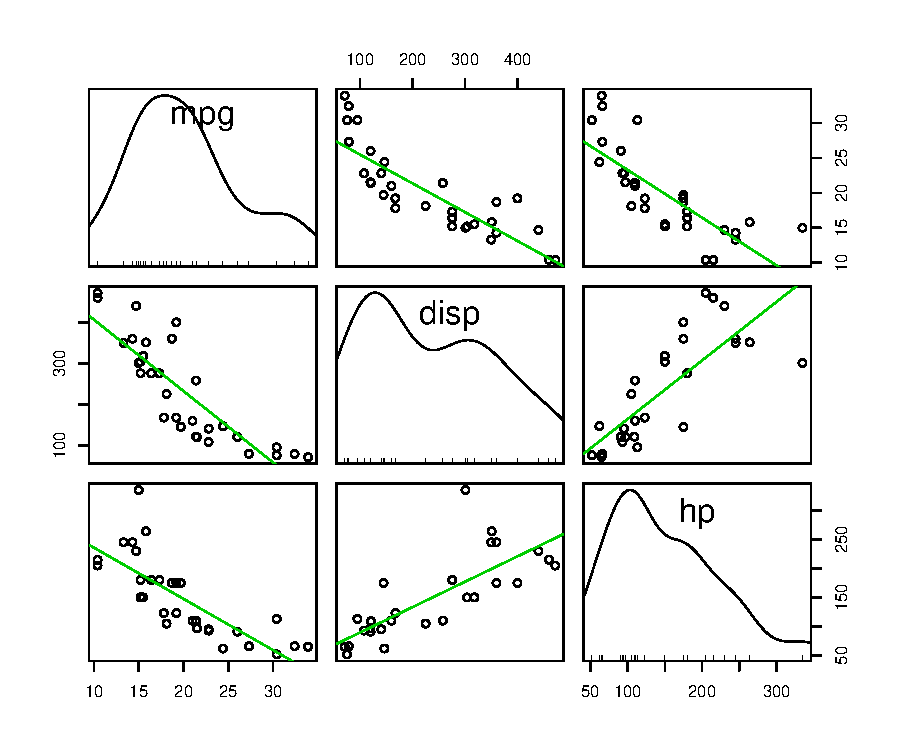
\includegraphics[width=1\linewidth]{figure/corplot-1} 

\end{knitrout}

\end{columns}

\end{frame}
%===============================================================================%


%===============================================================================%
\begin{frame}[t]{O processo de construção do modelo}
\begin{small}

1) Construa o seu modelo conceitual

2) Traduza suas hipóteses em modelos estatísticos

3) Colete seus dados

4) Faça uma análise exploratória 

5) ``Seleção de variáveis'' -  Avaliação das hipóteses \pause

\begin{itemize}
\small
\item Aqui, os seus modelos serão avaliados comparativamente \pause

\item Na maioria das vezes, as hipóteses são formuladas \emph{post hoc}, e as variáveis são adicionadas e removidas durante esse processo. Não é o ideal. \pause
\vfill
\item Você pretende \textbf{explicar} a relação entre as variáveis? Comece com o modelo completo e avalie os coeficientes e incertezas (erros e valores p). 


\end{small}
\end{itemize}
\end{frame}
%===============================================================================%


%===============================================================================%
\begin{frame}[t]{O processo de construção do modelo}
\begin{small}

1) Construa o seu modelo conceitual

2) Traduza suas hipóteses em modelos estatísticos

3) Colete seus dados

4) Faça uma análise exploratória 

5) ``Seleção de variáveis'' -  Avaliação das hipóteses 

\begin{itemize}

\item Cuidado com o efeito da multicolinearidade! Calcule os VIFs, e aplique medidas corretivas se necessário! \pause
\vfill
\item O objetivo é prever? Avalie a contribuição de cada variável para o modelo final, e mantenha só as mais importantes. Esta avaliação é mais robusta se houver validação independente.

\end{small}
\end{itemize}
\end{frame}
%===============================================================================%

%===============================================================================%
\begin{frame}{Seleção de variáveis}

Para cada conjunto de $k = p -1$ preditores, existem $2^{p-1}$ combinações de variáveis.
\pause
\vfill
Para que possamos determinar quais variáveis realmente contribuem para o modelo final, precisamos de uma medida objetiva. \pause
\vfill
Já conhecemos uma dessas medidas, o ... \pause $R^2 _{ajustado}$. \pause
\vfill
Podemos também usar os p-valores de cada coeficiente. \pause
\vfill
Mas, por causa da multicolinearidade, os p-valores podem esconder variáveis importantes, mas correlacionadas.

\end{frame}
%===============================================================================%

%===============================================================================%
\begin{frame}{AIC: Akaike's Information Criterion}

A medida conhecida como AIC (Akaike's Information Criterion) é a mais comumente usada para comparação de modelos. \pause
\vfill
O AIC é baseado no método de estimação por máxima verossimilhança, e na teoria da informação. \pause
\vfill
Definimos o AIC como:
\vfill
$2k - 2\ln(L)$
\vfill
$k$ é o número de parâmetros.
\vfill
$L$ é a função de verossimilhança. Minimizamos essa função para encontrar a reta do modelo.

\end{frame}
%===============================================================================%

%===============================================================================%
\begin{frame}{AIC: Akaike's Information Criterion}

Para a comparação de modelos estimados por OLS, podemos usar a função equivalente: 
\vfill
$AIC = 2k + n\log(SQ$_{Res}$/n)$ \pause
\vfill
Interpretação: 
\vfill
Quanto melhor o ajuste do modelo, menor é $\ln(L)$ ou $n\log(SQ_{Res}/n)$ \pause
\vfill
Mas quanto mais parâmetros adicionarmos, maior é $2k$ \pause
\vfill
O melhor modelo minimiza o valor do AIC, através de uma combinação entre bom ajuste e \textbf{parcimônia}.
\end{frame}
%===============================================================================%

%===============================================================================%
\begin{frame}[fragile]{Exemplo: AIC}

\begin{columns}[t]

\column{0.5\linewidth}
\setlength{\topsep}{2pt}
\begin{knitrout}\tiny
\definecolor{shadecolor}{rgb}{0.969, 0.969, 0.969}\color{fgcolor}\begin{kframe}
\begin{alltt}
\hlstd{m1} \hlkwb{<-} \hlkwd{lm}\hlstd{(qsec} \hlopt{~} \hlstd{hp,} \hlkwc{data}\hlstd{=mtcars)}
\hlkwd{summary}\hlstd{(m1)}\hlopt{$}\hlstd{r.squared}
\end{alltt}
\begin{verbatim}
## [1] 0.5015804
\end{verbatim}
\begin{alltt}
\hlkwd{summary}\hlstd{(m1)}\hlopt{$}\hlstd{adj.r.squared}
\end{alltt}
\begin{verbatim}
## [1] 0.4849664
\end{verbatim}
\begin{alltt}
\hlkwd{AIC}\hlstd{(m1)}
\end{alltt}
\begin{verbatim}
## [1] 110.6665
\end{verbatim}
\begin{alltt}
\hlcom{##}
\hlstd{m2} \hlkwb{<-} \hlkwd{lm}\hlstd{(qsec} \hlopt{~} \hlstd{hp} \hlopt{+} \hlstd{wt,} \hlkwc{data}\hlstd{=mtcars)}
\hlkwd{summary}\hlstd{(m2)}\hlopt{$}\hlstd{r.squared}
\end{alltt}
\begin{verbatim}
## [1] 0.6520291
\end{verbatim}
\begin{alltt}
\hlkwd{summary}\hlstd{(m2)}\hlopt{$}\hlstd{adj.r.squared}
\end{alltt}
\begin{verbatim}
## [1] 0.6280311
\end{verbatim}
\begin{alltt}
\hlkwd{AIC}\hlstd{(m1,m2)}
\end{alltt}
\begin{verbatim}
##    df      AIC
## m1  3 110.6665
## m2  4 101.1682
\end{verbatim}
\end{kframe}
\end{knitrout}

\column{0.5\linewidth}
\setlength{\topsep}{2pt}
\begin{knitrout}\tiny
\definecolor{shadecolor}{rgb}{0.969, 0.969, 0.969}\color{fgcolor}\begin{kframe}
\begin{alltt}
\hlstd{m3} \hlkwb{<-} \hlkwd{lm}\hlstd{(qsec} \hlopt{~} \hlstd{hp} \hlopt{+} \hlstd{wt} \hlopt{+} \hlstd{disp,} \hlkwc{data}\hlstd{=mtcars)}
\hlkwd{summary}\hlstd{(m3)}\hlopt{$}\hlstd{r.squared}
\end{alltt}
\begin{verbatim}
## [1] 0.6808292
\end{verbatim}
\begin{alltt}
\hlkwd{summary}\hlstd{(m3)}\hlopt{$}\hlstd{adj.r.squared}
\end{alltt}
\begin{verbatim}
## [1] 0.6466324
\end{verbatim}
\begin{alltt}
\hlkwd{AIC}\hlstd{(m1,m2,m3)}
\end{alltt}
\begin{verbatim}
##    df      AIC
## m1  3 110.6665
## m2  4 101.1682
## m3  5 100.4036
\end{verbatim}
\end{kframe}
\end{knitrout}
\end{columns}

\end{frame}
%===============================================================================%



%===============================================================================%
\begin{frame}{Observações Importantes}
\begin{small}

Outras medidas de comparação existem (Ex. AICc, BIC)
\vfill
Diferentemente de testes de significância (\emph{p-values} ou \emph{likelihood tests}), os modelos comparados por AIC, AICc ou BIC não precisam ser aninhados (\emph{nested}).
\vfill
Contudo, a  \textbf{variáveldependente e suas observações} precisam ser exatamente as mesmas. O que estamos avaliando e á capacidade de cada modelo em explicar/prever cada uma dessas variáveis.
\vfill
Uma alternativa à escolha de um único modelo é o método de \emph{model averaging}. Vários modelos são combinados, ponderados pela força da evidencia de cada um deles. \pause

A melhor seleção de variáveis sempre dependerá da concordância do modelo com a teoria, e da aplicação esperada. 
\vfill
Quem vai receber o título: você ou o computador?

\end{small}
\end{frame}
%===============================================================================%


%===============================================================================%
\begin{frame}{Leituras Importantes}

\begin{scriptsize}

Johnson JB, Omland KS (2004) Model selection in ecology and evolution. Trends in Ecology & Evolution, 19, 101–8.
\vfill
Whittingham MJ, Stephens P a, Bradbury RB, Freckleton RP (2006) Why do we still use stepwise modelling in ecology and behaviour? The Journal of Animal Ecology, 75, 1182–9.
 \vfill
Anderson D (2008) Model Based Inference in the Life Sciences: A Primer on Evidence. Springer New York, New York, NY, 146 pp.
\vfill
Burnham KP (2004) Multimodel Inference: Understanding AIC and BIC in Model Selection. Sociological Methods & Research, 33, 261–304.
\vfill
Anderson D, Burnham KP (2000) Null hypothesis testing: problems, prevalence, and an alternative. The Journal of Wildlife Management, 64, 912–923.

\end{scriptsize}

\end{frame}
%===============================================================================%

%===============================================================================%
\begin{frame}{Algoritmos de seleção de variáveis}

Existem métodos automáticos de seleção de variáveis (ex. \emph{stepwise}) 
\vfill
Tema da moda: \textbf{data mining} \pause
\vfill
Estes métodos podem oferecer contribuições importantes na \textbf{análise exploratória} do seu modelo. \pause
\vfill
Mas a melhor seleção final de variáveis sempre dependerá da concordância do modelo com a teoria, e da aplicação esperada. \pause
\vfill
Quem vai receber o diploma: voce ou o computador?

\end{frame}
%===============================================================================%


%===============================================================================%
\begin{frame}{Método \emph{Stepwise}}

\emph{Stepwise} significa passo a passo. \pause
\vfill
O método pode ser aplicado de maneira crescente (\emph{forward}) ou decrescente (\emph{backward}). \pause
\vfill
No modo \emph{forward}, começamos com uma única variável, e vamos progressivamente adicionando mais variáveis, testando o ganho em poder explicativo a cada nova adição. \pause
\vfill
No modo \emph{backward}, começamos com todas as variáveis, e vamos progressivamente eliminando cada uma, testando a perda em poder explicativo a cada nova adição.

\end{frame}
%===============================================================================%



%===============================================================================%
\begin{frame}{Método \emph{Stepwise}}

O método usado para calcular esse "ganho" ou "perda" de informação pode variar de acordo com a escolha do usuário \pause
\vfill
O método stepwise original é baseado em testes F de significância, e bastante criticado por sua ampla sensitividade à multicolinearidade. \pause
\vfill
O uso de medidas mais robustas como o AIC reduzem, mas não eliminam, esse problema. \pause
\vfill
Quando duas variáveis são muito parecidas, a escolha se torna arbitrária, e somente o suporte teórico (i.e. bom senso) pode resolver o problema.

\end{frame}
%===============================================================================%


%===============================================================================%
\begin{frame}[fragile]{Método \emph{Stepwise}}

\begin{columns}

\column{0.5\linewidth}
\setlength{\topsep}{2pt}
\begin{knitrout}\tiny
\definecolor{shadecolor}{rgb}{0.969, 0.969, 0.969}\color{fgcolor}\begin{kframe}
\begin{alltt}
\hlstd{form} \hlkwb{<-} \hlkwd{vector}\hlstd{()}

\hlkwa{for}\hlstd{(i} \hlkwa{in} \hlkwd{c}\hlstd{(}\hlnum{1}\hlopt{:}\hlnum{100}\hlstd{))\{}
    \hlstd{x1} \hlkwb{<-} \hlkwd{runif}\hlstd{(}\hlnum{30}\hlstd{,}\hlnum{0}\hlstd{,}\hlnum{20}\hlstd{)}
    \hlstd{x2} \hlkwb{<-} \hlstd{x1} \hlopt{+} \hlkwd{rnorm}\hlstd{(}\hlnum{30}\hlstd{,}\hlnum{0}\hlstd{,}\hlnum{1}\hlstd{)}
    \hlstd{y} \hlkwb{<-} \hlnum{3} \hlopt{+} \hlnum{2.3}\hlopt{*}\hlstd{x1} \hlopt{+} \hlnum{2.1}\hlopt{*}\hlstd{x2} \hlopt{+} \hlkwd{rnorm}\hlstd{(}\hlnum{30}\hlstd{,}\hlnum{0}\hlstd{,}\hlnum{10}\hlstd{)}
    \hlstd{m} \hlkwb{<-} \hlkwd{lm}\hlstd{(y} \hlopt{~} \hlstd{x1} \hlopt{+} \hlstd{x2)}
    \hlstd{sm} \hlkwb{<-} \hlkwd{step}\hlstd{(m,} \hlkwc{trace}\hlstd{=}\hlnum{0}\hlstd{)}
    \hlstd{form} \hlkwb{<-} \hlkwd{c}\hlstd{(form,} \hlkwd{as.character}\hlstd{(}\hlkwd{formula}\hlstd{(sm))[}\hlnum{3}\hlstd{])}
  \hlstd{\}}

\hlkwd{barplot}\hlstd{(}\hlkwd{table}\hlstd{(}\hlkwd{factor}\hlstd{(form)))}
\end{alltt}
\end{kframe}
\end{knitrout}

\column{0.6\linewidth}

\begin{knitrout}
\definecolor{shadecolor}{rgb}{0.969, 0.969, 0.969}\color{fgcolor}
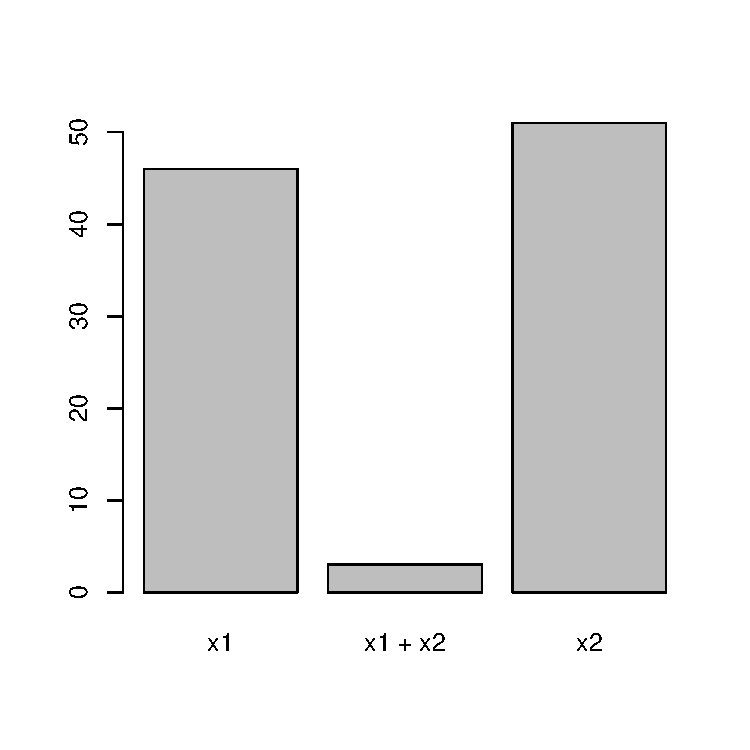
\includegraphics[width=1\linewidth]{figure/stepburrop-1} 

\end{knitrout}

\end{columns}

\end{frame}
%===============================================================================%


%===============================================================================%
\begin{frame}[fragile]{Método \emph{Stepwise}}

Uma alternativa interessante pode ser combinar o método \emph{stepwise} com métodos de aleatorização. Mas mesmo assim, continua sendo uma análise exploratória.

\vfill


\begin{knitrout}\tiny
\definecolor{shadecolor}{rgb}{0.969, 0.969, 0.969}\color{fgcolor}\begin{kframe}
\begin{alltt}
\hlstd{m1} \hlkwb{<-} \hlkwd{lm} \hlstd{(qsec} \hlopt{~} \hlstd{., mtcars)}

\hlkwd{library}\hlstd{(bootStepAIC)}
\end{alltt}


{\ttfamily\noindent\itshape\color{messagecolor}{\#\# Loading required package: MASS}}\begin{alltt}
\hlstd{m.boot} \hlkwb{<-} \hlkwd{boot.stepAIC}\hlstd{(m1,mtcars,}\hlkwc{B} \hlstd{=} \hlnum{10}\hlstd{,} \hlkwc{direction}\hlstd{=}\hlstr{"both"}\hlstd{)}
\end{alltt}
\end{kframe}
\end{knitrout}

\end{frame}
%===============================================================================%

%===============================================================================%
\begin{frame}[fragile]{Método \emph{Stepwise}}

\begin{knitrout}\tiny
\definecolor{shadecolor}{rgb}{0.969, 0.969, 0.969}\color{fgcolor}\begin{kframe}
\begin{alltt}
\hlstd{m.boot}\hlopt{$}\hlstd{Covariates}
\end{alltt}
\begin{verbatim}
##      (%)
## wt   100
## gear  90
## am    80
## vs    80
## cyl   70
## hp    70
## disp  60
## mpg   60
## carb  20
## drat  20
\end{verbatim}
\end{kframe}
\end{knitrout}

\end{frame}
%===============================================================================%


%===============================================================================%
\begin{frame}[fragile]{Método \emph{Stepwise}}

\begin{knitrout}\tiny
\definecolor{shadecolor}{rgb}{0.969, 0.969, 0.969}\color{fgcolor}\begin{kframe}
\begin{alltt}
\hlstd{m.boot}\hlopt{$}\hlstd{Sign}
\end{alltt}
\begin{verbatim}
##          + (%)     - (%)
## mpg  100.00000   0.00000
## vs   100.00000   0.00000
## wt   100.00000   0.00000
## hp    28.57143  71.42857
## am    12.50000  87.50000
## gear  11.11111  88.88889
## carb   0.00000 100.00000
## cyl    0.00000 100.00000
## disp   0.00000 100.00000
## drat   0.00000 100.00000
\end{verbatim}
\end{kframe}
\end{knitrout}

\end{frame}
%===============================================================================%


%===============================================================================%
\begin{frame}[fragile]{Método \emph{Stepwise}}

\begin{knitrout}\tiny
\definecolor{shadecolor}{rgb}{0.969, 0.969, 0.969}\color{fgcolor}\begin{kframe}
\begin{alltt}
\hlstd{m.boot}\hlopt{$}\hlstd{Significance}
\end{alltt}
\begin{verbatim}
##            (%)
## carb 100.00000
## wt   100.00000
## gear  88.88889
## vs    87.50000
## cyl   85.71429
## disp  83.33333
## am    75.00000
## mpg   66.66667
## hp    57.14286
## drat  50.00000
\end{verbatim}
\end{kframe}
\end{knitrout}

\end{frame}
%===============================================================================%


%===============================================================================%
\begin{frame}[fragile]{Método \emph{Stepwise}}

\begin{knitrout}\tiny
\definecolor{shadecolor}{rgb}{0.969, 0.969, 0.969}\color{fgcolor}\begin{kframe}
\begin{alltt}
\hlstd{m.boot[}\hlnum{4}\hlopt{:}\hlnum{6}\hlstd{]}
\end{alltt}
\begin{verbatim}
## $OrigModel
## 
## Call:
## lm(formula = qsec ~ ., data = mtcars)
## 
## Coefficients:
## (Intercept)          mpg          cyl         disp           hp         drat  
##   17.776177     0.069048    -0.362678    -0.007501    -0.001563    -0.131064  
##          wt           vs           am         gear         carb  
##    1.496332     0.970035    -0.901186    -0.201285    -0.273598  
## 
## 
## $OrigStepAIC
## 
## Call:
## lm(formula = qsec ~ cyl + disp + wt + vs + am + carb, data = mtcars)
## 
## Coefficients:
## (Intercept)          cyl         disp           wt           vs           am  
##   18.611144    -0.369984    -0.008899     1.475086     0.968162    -0.902579  
##        carb  
##   -0.434722  
## 
## 
## $direction
## [1] "both"
\end{verbatim}
\end{kframe}
\end{knitrout}

\end{frame}
%===============================================================================%


%===============================================================================%
\begin{frame}[fragile]{Método \emph{Stepwise}}

\begin{knitrout}\tiny
\definecolor{shadecolor}{rgb}{0.969, 0.969, 0.969}\color{fgcolor}\begin{kframe}
\begin{alltt}
\hlstd{m.boot[}\hlnum{7}\hlopt{:}\hlnum{8}\hlstd{]}
\end{alltt}
\begin{verbatim}
## $k
## [1] 2
## 
## $BootStepAIC
## $BootStepAIC[[1]]
## 
## Call:
## lm(formula = qsec ~ cyl + hp + wt + vs + gear, data = boot.data)
## 
## Coefficients:
## (Intercept)          cyl           hp           wt           vs         gear  
##    20.55994     -0.29160     -0.01034      0.68602      1.42131     -0.63289  
## 
## 
## $BootStepAIC[[2]]
## 
## Call:
## lm(formula = qsec ~ mpg + cyl + disp + wt + vs + am + gear, data = boot.data)
## 
## Coefficients:
## (Intercept)          mpg          cyl         disp           wt           vs  
##    19.66381      0.09939     -0.47900     -0.00653      1.02154      0.86578  
##          am         gear  
##    -1.35078     -0.65210  
## 
## 
## $BootStepAIC[[3]]
## 
## Call:
## lm(formula = qsec ~ mpg + disp + wt + vs + am + carb, data = boot.data)
## 
## Coefficients:
## (Intercept)          mpg         disp           wt           vs           am  
##    12.27735      0.13431     -0.01449      2.35212      0.98014     -0.97029  
##        carb  
##    -0.48150  
## 
## 
## $BootStepAIC[[4]]
## 
## Call:
## lm(formula = qsec ~ mpg + cyl + disp + hp + wt + am + gear, data = boot.data)
## 
## Coefficients:
## (Intercept)          mpg          cyl         disp           hp           wt  
##    20.40077      0.19651     -0.91795     -0.01578      0.01145      1.89897  
##          am         gear  
##    -1.86269     -1.18415  
## 
## 
## $BootStepAIC[[5]]
## 
## Call:
## lm(formula = qsec ~ cyl + hp + wt + vs + am + gear, data = boot.data)
## 
## Coefficients:
## (Intercept)          cyl           hp           wt           vs           am  
##    21.60199     -0.31542     -0.01264      0.66081      1.24630     -0.25738  
##        gear  
##    -0.73669  
## 
## 
## $BootStepAIC[[6]]
## 
## Call:
## lm(formula = qsec ~ cyl + disp + hp + wt + am + gear, data = boot.data)
## 
## Coefficients:
## (Intercept)          cyl         disp           hp           wt           am  
##    31.88777     -1.47260     -0.01160      0.01134      1.10371     -1.80027  
##        gear  
##    -1.77283  
## 
## 
## $BootStepAIC[[7]]
## 
## Call:
## lm(formula = qsec ~ cyl + wt + vs + am + gear, data = boot.data)
## 
## Coefficients:
## (Intercept)          cyl           wt           vs           am         gear  
##     24.0230      -0.8402       0.4179       0.9296      -1.5563      -0.5644  
## 
## 
## $BootStepAIC[[8]]
## 
## Call:
## lm(formula = qsec ~ mpg + hp + drat + wt + vs + am + gear, data = boot.data)
## 
## Coefficients:
## (Intercept)          mpg           hp         drat           wt           vs  
##   15.452675     0.162334    -0.009411    -0.909752     1.205355     1.995387  
##          am         gear  
##    0.459485    -0.334018  
## 
## 
## $BootStepAIC[[9]]
## 
## Call:
## lm(formula = qsec ~ mpg + cyl + disp + hp + drat + wt + vs + 
##     am + gear, data = boot.data)
## 
## Coefficients:
## (Intercept)          mpg          cyl         disp           hp         drat  
##   11.654973     0.116489    -0.240142    -0.006717    -0.014728    -0.384375  
##          wt           vs           am         gear  
##    1.598091     1.088756    -3.358608     1.817977  
## 
## 
## $BootStepAIC[[10]]
## 
## Call:
## lm(formula = qsec ~ mpg + disp + hp + wt + vs + gear + carb, 
##     data = boot.data)
## 
## Coefficients:
## (Intercept)          mpg         disp           hp           wt           vs  
##   16.831180     0.060837    -0.007934    -0.008131     1.546590     1.143890  
##        gear         carb  
##   -0.547627    -0.270338
\end{verbatim}
\end{kframe}
\end{knitrout}

\end{frame}
%===============================================================================%


\section{Mais extensões dos modelos lineares gerais}

%===============================================================================%
\begin{frame}[fragile]{Regressão Polinomial}

\begin{columns}

\column{0.5\linewidth}
\setlength{\topsep}{2pt}
\begin{knitrout}\tiny
\definecolor{shadecolor}{rgb}{0.969, 0.969, 0.969}\color{fgcolor}\begin{kframe}
\begin{alltt}
\hlkwd{set.seed}\hlstd{(}\hlnum{234}\hlstd{)}

\hlstd{x} \hlkwb{<-} \hlkwd{runif}\hlstd{(}\hlnum{50}\hlstd{,}\hlnum{0}\hlstd{,}\hlnum{50}\hlstd{)}

\hlstd{y} \hlkwb{<-} \hlnum{5} \hlopt{+} \hlnum{1.3}\hlopt{*}\hlstd{x} \hlopt{+} \hlnum{0.5}\hlopt{*}\hlstd{x}\hlopt{^}\hlnum{2} \hlopt{+} \hlkwd{rnorm}\hlstd{(}\hlnum{50}\hlstd{,}\hlnum{0}\hlstd{,}\hlnum{100}\hlstd{)}

\hlstd{m} \hlkwb{<-} \hlkwd{lm}\hlstd{(y} \hlopt{~} \hlstd{x} \hlopt{+} \hlkwd{I}\hlstd{(x}\hlopt{^}\hlnum{2}\hlstd{))}

\hlkwd{plot}\hlstd{(x,y,} \hlkwc{pch}\hlstd{=}\hlnum{19}\hlstd{)}

\hlstd{xnovo} \hlkwb{<-} \hlkwd{data.frame}\hlstd{(} \hlkwc{x} \hlstd{=} \hlkwd{seq}\hlstd{(}\hlnum{0}\hlstd{,}\hlnum{50}\hlstd{,}\hlkwc{by}\hlstd{=}\hlnum{0.5}\hlstd{))}

\hlstd{p} \hlkwb{<-} \hlkwd{predict}\hlstd{(m,xnovo)}

\hlkwd{lines}\hlstd{(xnovo[,}\hlnum{1}\hlstd{],p,} \hlkwc{lwd}\hlstd{=}\hlnum{2}\hlstd{,}\hlkwc{col}\hlstd{=}\hlstr{'red'}\hlstd{)}
\end{alltt}
\end{kframe}
\end{knitrout}

\column{0.5\linewidth}

\begin{knitrout}
\definecolor{shadecolor}{rgb}{0.969, 0.969, 0.969}\color{fgcolor}
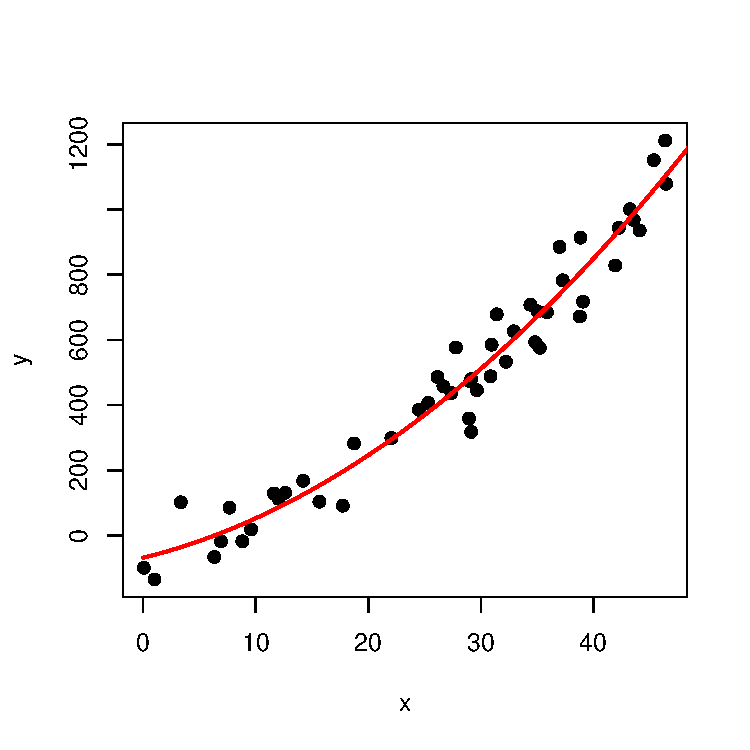
\includegraphics[width=1\linewidth]{figure/samppol2plot-1} 

\end{knitrout}


\end{columns}

\end{frame}
%===============================================================================%

%===============================================================================%
\begin{frame}[fragile]{Regressão Polinomial}

\begin{columns}

\column{0.5\linewidth}
\setlength{\topsep}{2pt}
\begin{knitrout}\tiny
\definecolor{shadecolor}{rgb}{0.969, 0.969, 0.969}\color{fgcolor}\begin{kframe}
\begin{alltt}
\hlkwd{set.seed}\hlstd{(}\hlnum{234}\hlstd{)}

\hlstd{x} \hlkwb{<-} \hlkwd{seq}\hlstd{(}\hlnum{2}\hlstd{,}\hlnum{10}\hlstd{,}\hlkwc{by}\hlstd{=}\hlnum{0.1}\hlstd{)}

\hlstd{y} \hlkwb{<-} \hlnum{3} \hlopt{+} \hlnum{2}\hlopt{*}\hlkwd{sin}\hlstd{(x)} \hlopt{+} \hlkwd{rnorm}\hlstd{(}\hlnum{81}\hlstd{,}\hlnum{0}\hlstd{,}\hlnum{1}\hlstd{)}

\hlstd{m} \hlkwb{<-} \hlkwd{lm}\hlstd{(y} \hlopt{~} \hlkwd{poly}\hlstd{(x,}\hlnum{3}\hlstd{))}

\hlkwd{plot}\hlstd{(x,y,} \hlkwc{pch}\hlstd{=}\hlnum{19}\hlstd{)}

\hlstd{xnovo} \hlkwb{<-} \hlkwd{data.frame}\hlstd{(} \hlkwc{x} \hlstd{=} \hlkwd{seq}\hlstd{(}\hlnum{2}\hlstd{,}\hlnum{10}\hlstd{,}\hlkwc{by}\hlstd{=}\hlnum{0.1}\hlstd{))}

\hlstd{p} \hlkwb{<-} \hlkwd{predict}\hlstd{(m,xnovo)}

\hlkwd{lines}\hlstd{(xnovo[,}\hlnum{1}\hlstd{],p,} \hlkwc{lwd}\hlstd{=}\hlnum{2}\hlstd{,}\hlkwc{col}\hlstd{=}\hlstr{'red'}\hlstd{)}
\end{alltt}
\end{kframe}
\end{knitrout}

\column{0.5\linewidth}

\begin{knitrout}
\definecolor{shadecolor}{rgb}{0.969, 0.969, 0.969}\color{fgcolor}
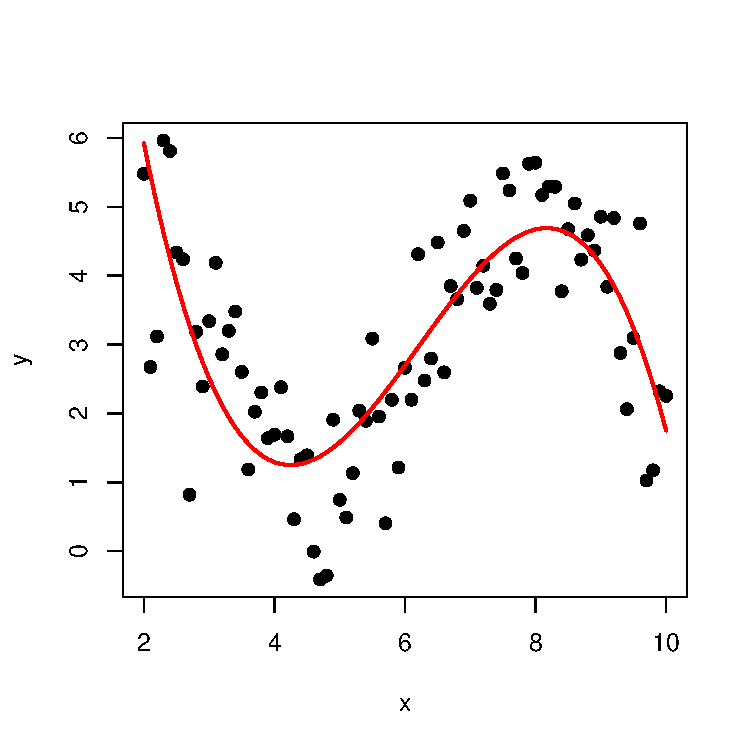
\includegraphics[width=1\linewidth]{figure/samppol3plot-1} 

\end{knitrout}


\end{columns}

\end{frame}
%===============================================================================%


%===============================================================================%
\begin{frame}[fragile]{Regressão Polinomial}

 Cuidado com polinômios exagerados!

\begin{columns}

\column{0.5\linewidth}
\setlength{\topsep}{2pt}
\begin{knitrout}\tiny
\definecolor{shadecolor}{rgb}{0.969, 0.969, 0.969}\color{fgcolor}\begin{kframe}
\begin{alltt}
\hlkwd{set.seed}\hlstd{(}\hlnum{234}\hlstd{)}

\hlstd{x} \hlkwb{<-} \hlkwd{seq}\hlstd{(}\hlnum{2}\hlstd{,}\hlnum{10}\hlstd{,}\hlkwc{by}\hlstd{=}\hlnum{0.1}\hlstd{)}

\hlstd{y} \hlkwb{<-} \hlnum{3} \hlopt{+} \hlnum{2}\hlopt{*}\hlkwd{sin}\hlstd{(x)} \hlopt{+} \hlkwd{rnorm}\hlstd{(}\hlnum{81}\hlstd{,}\hlnum{0}\hlstd{,}\hlnum{1}\hlstd{)}

\hlstd{m} \hlkwb{<-} \hlkwd{lm}\hlstd{(y} \hlopt{~} \hlkwd{poly}\hlstd{(x,}\hlnum{20}\hlstd{))}

\hlkwd{plot}\hlstd{(x,y,} \hlkwc{pch}\hlstd{=}\hlnum{19}\hlstd{)}

\hlstd{xnovo} \hlkwb{<-} \hlkwd{data.frame}\hlstd{(} \hlkwc{x} \hlstd{=} \hlkwd{seq}\hlstd{(}\hlnum{2}\hlstd{,}\hlnum{10}\hlstd{,}\hlkwc{by}\hlstd{=}\hlnum{0.1}\hlstd{))}

\hlstd{p} \hlkwb{<-} \hlkwd{predict}\hlstd{(m,xnovo)}

\hlkwd{lines}\hlstd{(xnovo[,}\hlnum{1}\hlstd{],p,} \hlkwc{lwd}\hlstd{=}\hlnum{2}\hlstd{,}\hlkwc{col}\hlstd{=}\hlstr{'red'}\hlstd{)}
\end{alltt}
\end{kframe}
\end{knitrout}

\column{0.5\linewidth}

\begin{knitrout}
\definecolor{shadecolor}{rgb}{0.969, 0.969, 0.969}\color{fgcolor}
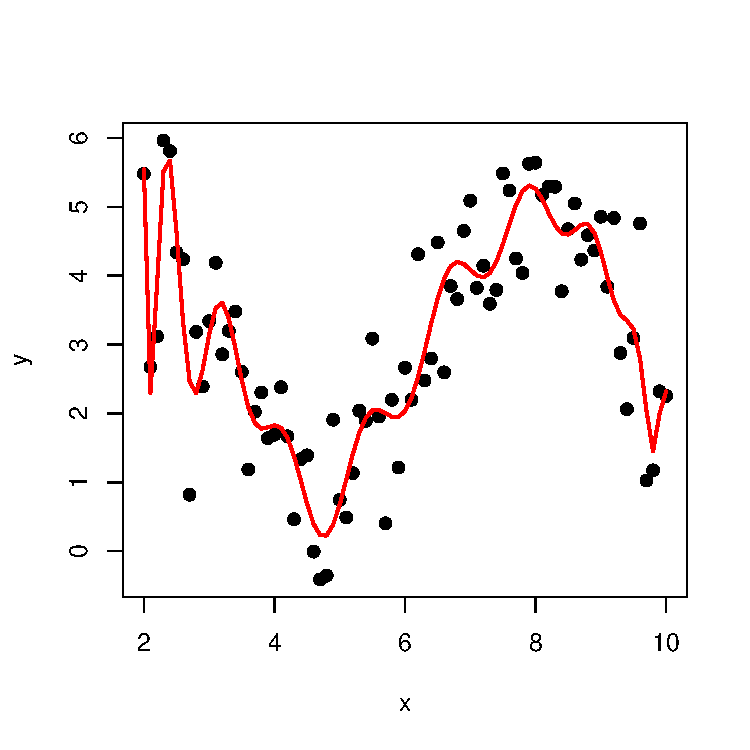
\includegraphics[width=1\linewidth]{figure/samppol20plot-1} 

\end{knitrout}


\end{columns}

\end{frame}
%===============================================================================%


%===============================================================================%
\begin{frame}{Regressão Polinomial}

Como saber se um modelo polinomial é melhor do que um modelo linear, e onde parar?
\vfill
\begin{itemize}
\item Não podemos usar $R^2$, porque ele sempre aumenta... \pause
\vfill
\item Não podemos usar $SQ_{reg}$, porque os residuos ficam cada vez menores com mais termos \pause
\vfill
\item Mas podemos usar o AIC!

\end{itemize}

\end{frame}
%===============================================================================%



%===============================================================================%
\begin{frame}[fragile]{Regressão Polinomial}

\begin{columns}

\column{0.5\linewidth}
\setlength{\topsep}{2pt}

\begin{knitrout}\tiny
\definecolor{shadecolor}{rgb}{0.969, 0.969, 0.969}\color{fgcolor}\begin{kframe}
\begin{alltt}
\hlkwd{set.seed}\hlstd{(}\hlnum{234}\hlstd{)}
\hlstd{x} \hlkwb{<-} \hlkwd{runif}\hlstd{(}\hlnum{50}\hlstd{,}\hlnum{0}\hlstd{,}\hlnum{50}\hlstd{)}
\hlstd{y} \hlkwb{<-} \hlnum{5} \hlopt{+} \hlnum{1.3}\hlopt{*}\hlstd{x} \hlopt{+} \hlnum{0.5}\hlopt{*}\hlstd{x}\hlopt{^}\hlnum{2} \hlopt{+} \hlkwd{rnorm}\hlstd{(}\hlnum{50}\hlstd{,}\hlnum{0}\hlstd{,}\hlnum{100}\hlstd{)}

\hlstd{m1} \hlkwb{<-} \hlkwd{lm}\hlstd{(y} \hlopt{~} \hlstd{x)}

\hlkwd{AIC}\hlstd{(m1)}
\end{alltt}
\begin{verbatim}
## [1] 602.9227
\end{verbatim}
\end{kframe}
\end{knitrout}

\column{0.5\linewidth}

\begin{knitrout}
\definecolor{shadecolor}{rgb}{0.969, 0.969, 0.969}\color{fgcolor}
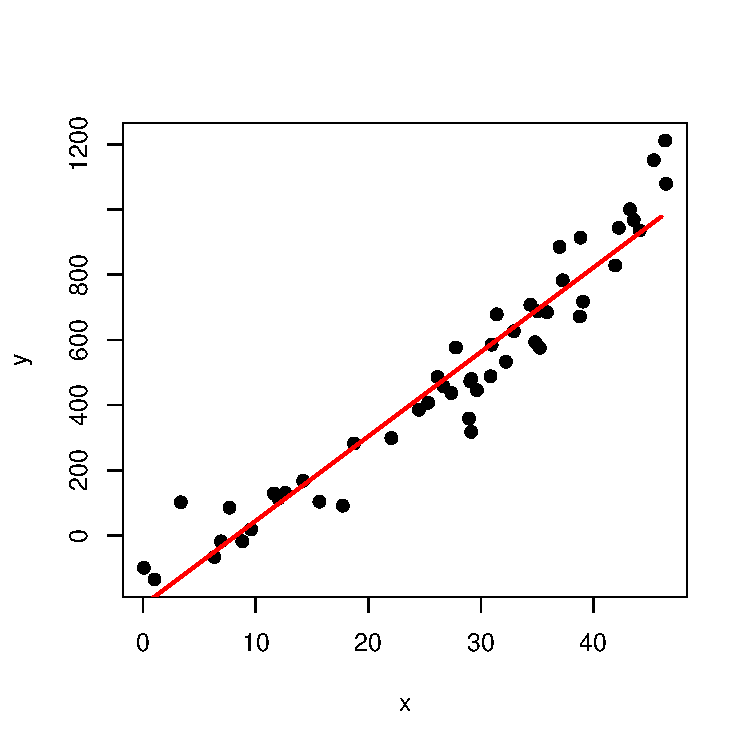
\includegraphics[width=1\linewidth]{figure/samppolallplot-1} 

\end{knitrout}

\end{columns}

\end{frame}
%===============================================================================%


%===============================================================================%
\begin{frame}[fragile]{Regressão Polinomial}

\begin{columns}

\column{0.5\linewidth}
\setlength{\topsep}{2pt}

\begin{knitrout}\tiny
\definecolor{shadecolor}{rgb}{0.969, 0.969, 0.969}\color{fgcolor}\begin{kframe}
\begin{alltt}
\hlstd{m2} \hlkwb{<-} \hlkwd{lm}\hlstd{(y} \hlopt{~} \hlkwd{poly}\hlstd{(x,}\hlnum{2}\hlstd{))}

\hlkwd{AIC}\hlstd{(m1,m2)}
\end{alltt}
\begin{verbatim}
##    df      AIC
## m1  3 602.9227
## m2  4 580.6495
\end{verbatim}
\end{kframe}
\end{knitrout}

\column{0.5\linewidth}

\begin{knitrout}
\definecolor{shadecolor}{rgb}{0.969, 0.969, 0.969}\color{fgcolor}
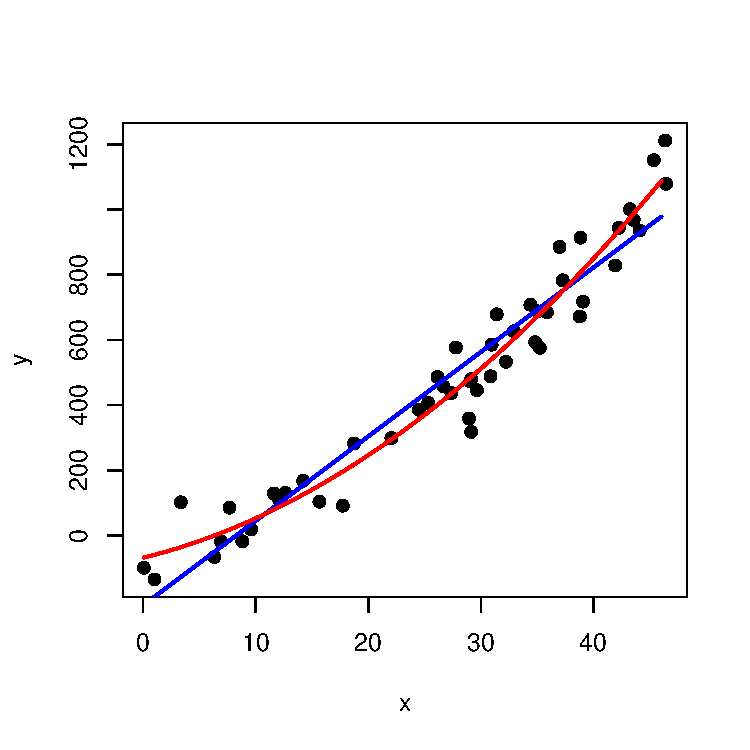
\includegraphics[width=1\linewidth]{figure/samppolallplot2-1} 

\end{knitrout}

\end{columns}

\end{frame}
%===============================================================================%


%===============================================================================%
\begin{frame}[fragile]{Regressão Polinomial}

\begin{columns}

\column{0.5\linewidth}
\setlength{\topsep}{2pt}

\begin{knitrout}\tiny
\definecolor{shadecolor}{rgb}{0.969, 0.969, 0.969}\color{fgcolor}\begin{kframe}
\begin{alltt}
\hlstd{m3} \hlkwb{<-} \hlkwd{lm}\hlstd{(y} \hlopt{~} \hlkwd{poly}\hlstd{(x,}\hlnum{3}\hlstd{))}


\hlkwd{AIC}\hlstd{(m1,m2,m3)}
\end{alltt}
\begin{verbatim}
##    df      AIC
## m1  3 602.9227
## m2  4 580.6495
## m3  5 581.8052
\end{verbatim}
\end{kframe}
\end{knitrout}

\column{0.5\linewidth}

\begin{knitrout}
\definecolor{shadecolor}{rgb}{0.969, 0.969, 0.969}\color{fgcolor}
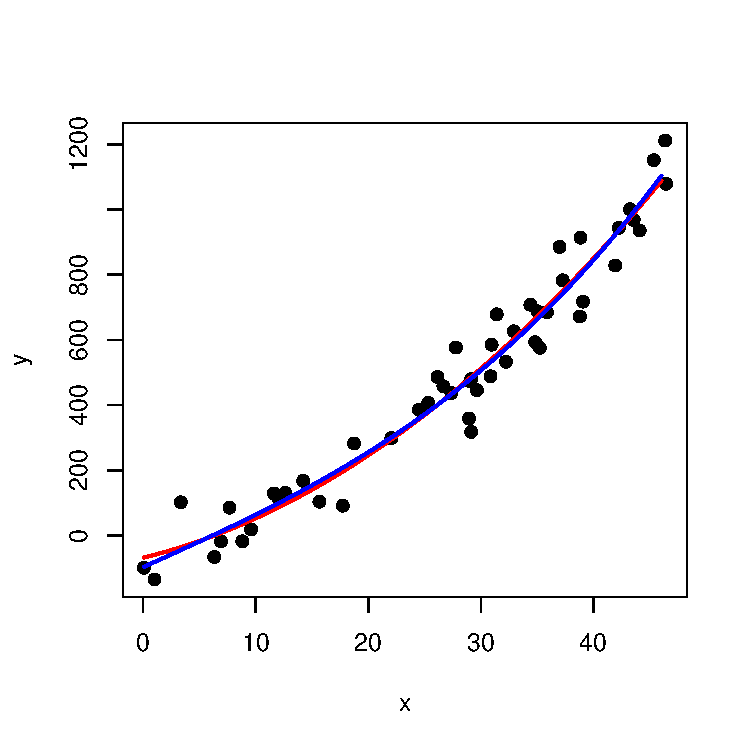
\includegraphics[width=1\linewidth]{figure/samppolallplot3-1} 

\end{knitrout}

\end{columns}

\end{frame}
%===============================================================================%


%===============================================================================%
\begin{frame}[fragile]{Regressão Polinomial}

\begin{columns}

\column{0.5\linewidth}
\setlength{\topsep}{2pt}

\begin{knitrout}\tiny
\definecolor{shadecolor}{rgb}{0.969, 0.969, 0.969}\color{fgcolor}\begin{kframe}
\begin{alltt}
\hlstd{m10} \hlkwb{<-} \hlkwd{lm}\hlstd{(y} \hlopt{~}\hlkwd{poly}\hlstd{(x,}\hlnum{10}\hlstd{))}

\hlkwd{AIC}\hlstd{(m1,m2,m3,m10)}
\end{alltt}
\begin{verbatim}
##     df      AIC
## m1   3 602.9227
## m2   4 580.6495
## m3   5 581.8052
## m10 12 592.0629
\end{verbatim}
\end{kframe}
\end{knitrout}

\column{0.5\linewidth}

\begin{knitrout}
\definecolor{shadecolor}{rgb}{0.969, 0.969, 0.969}\color{fgcolor}
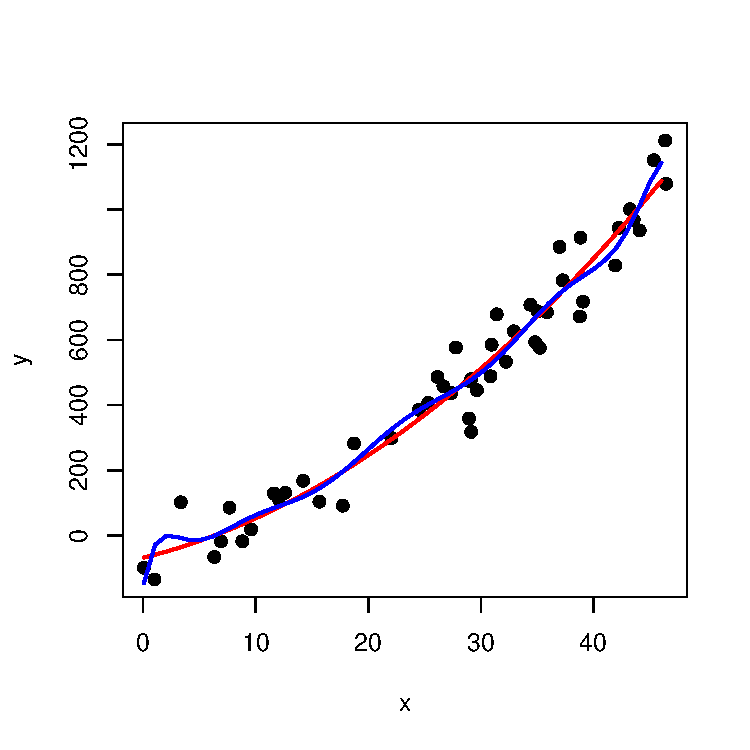
\includegraphics[width=1\linewidth]{figure/samppolallplot4-1} 

\end{knitrout}

\end{columns}

\end{frame}
%===============================================================================%

%===============================================================================%
\begin{frame}{Regressão Polinomial}

Limitações dos modelos polinomiais
\vfill
\begin{itemize}
\item Os coeficientes não tem uma interpreteção direta \pause
\vfill 
 \begin{itemize}
    \item Não posso manter $X _1$ constante e variar $X _$ \pause
  \end{itemize}
\vfill
\item Extrapolações são muito pouco confiáveis, pois o efeito dos termos de potência é muito forte fora do escopo
\end{itemize}

\end{frame}
%===============================================================================%


%===============================================================================%
\begin{frame}{Regressão Normalizada}

Para comparação de coeficientes com unidades diferentes
\vfill
\begin{itemize}
\item Obtida através de normalização das variáveis: \pause
\vfill
\item \dfrac{X - \bar X}{s} \pause
\vfill
\item A subtração da média é chamada de \textbf{centralização} dos dados\pause
\vfill
\item A divisão pelo desvio padrão fornece a \textbf{normalização} da variância \pause
\vfill
\item Bônus: A estimativa de $\beta _0$ se torna o valor de $E(Y)$ para os valores médios de $X$
\end{itemize}

\end{frame}
%===============================================================================%


%===============================================================================%
\begin{frame}[fragile]{Regressão Normalizada}

\begin{columns}

\column{0.5\linewidth}
\setlength{\topsep}{2pt}
\begin{knitrout}\tiny
\definecolor{shadecolor}{rgb}{0.969, 0.969, 0.969}\color{fgcolor}\begin{kframe}
\begin{alltt}
\hlstd{x1} \hlkwb{<-} \hlkwd{runif}\hlstd{(}\hlnum{20}\hlstd{,}\hlnum{0}\hlstd{,}\hlnum{100}\hlstd{)}
\hlstd{x2} \hlkwb{<-} \hlkwd{runif}\hlstd{(}\hlnum{20}\hlstd{,}\hlnum{0}\hlstd{,}\hlnum{10}\hlstd{)}
\hlstd{y} \hlkwb{<-} \hlnum{5} \hlopt{+} \hlnum{3}\hlopt{*}\hlstd{x1} \hlopt{+} \hlnum{30}\hlopt{*}\hlstd{x2} \hlopt{+} \hlkwd{rnorm}\hlstd{(}\hlnum{20}\hlstd{,}\hlnum{0}\hlstd{,}\hlnum{20}\hlstd{)}
\hlstd{m} \hlkwb{<-} \hlkwd{lm}\hlstd{(y} \hlopt{~} \hlstd{x1} \hlopt{+} \hlstd{x2)}
\hlkwd{summary}\hlstd{(m)}
\end{alltt}
\begin{verbatim}
## 
## Call:
## lm(formula = y ~ x1 + x2)
## 
## Residuals:
##     Min      1Q  Median      3Q     Max 
## -49.956  -9.722   5.638  12.781  27.107 
## 
## Coefficients:
##             Estimate Std. Error t value Pr(>|t|)    
## (Intercept)   2.2083    12.2693    0.18    0.859    
## x1            3.1714     0.1787   17.75 2.09e-12 ***
## x2           28.0824     1.8342   15.31 2.24e-11 ***
## ---
## Signif. codes:  0 '***' 0.001 '**' 0.01 '*' 0.05 '.' 0.1 ' ' 1
## 
## Residual standard error: 22.95 on 17 degrees of freedom
## Multiple R-squared:  0.9741,	Adjusted R-squared:  0.9711 
## F-statistic: 320.1 on 2 and 17 DF,  p-value: 3.227e-14
\end{verbatim}
\end{kframe}
\end{knitrout}

\column{0.5\linewidth}
\setlength{\topsep}{2pt}
\begin{knitrout}\tiny
\definecolor{shadecolor}{rgb}{0.969, 0.969, 0.969}\color{fgcolor}\begin{kframe}
\begin{alltt}
\hlstd{x1n} \hlkwb{<-} \hlstd{(x1}\hlopt{-}\hlkwd{mean}\hlstd{(x1))}\hlopt{/}\hlkwd{sd}\hlstd{(x1)}
\hlstd{x2n} \hlkwb{<-} \hlstd{(x2}\hlopt{-}\hlkwd{mean}\hlstd{(x2))}\hlopt{/}\hlkwd{sd}\hlstd{(x2)}
\hlstd{mn} \hlkwb{<-} \hlkwd{lm}\hlstd{(y} \hlopt{~} \hlstd{x1n} \hlopt{+} \hlstd{x2n)}
\hlkwd{summary}\hlstd{(mn)}
\end{alltt}
\begin{verbatim}
## 
## Call:
## lm(formula = y ~ x1n + x2n)
## 
## Residuals:
##     Min      1Q  Median      3Q     Max 
## -49.956  -9.722   5.638  12.781  27.107 
## 
## Coefficients:
##             Estimate Std. Error t value Pr(>|t|)    
## (Intercept)  280.077      5.131   54.59  < 2e-16 ***
## x1n           94.397      5.319   17.75 2.09e-12 ***
## x2n           81.430      5.319   15.31 2.24e-11 ***
## ---
## Signif. codes:  0 '***' 0.001 '**' 0.01 '*' 0.05 '.' 0.1 ' ' 1
## 
## Residual standard error: 22.95 on 17 degrees of freedom
## Multiple R-squared:  0.9741,	Adjusted R-squared:  0.9711 
## F-statistic: 320.1 on 2 and 17 DF,  p-value: 3.227e-14
\end{verbatim}
\end{kframe}
\end{knitrout}


\end{columns}

\end{frame}
%===============================================================================%

\section{Modelos Lineares Generalizados}

%===============================================================================%
\begin{frame}{Regressão Logística}

A \textbf{Regressão Logística} inverte o jogo, e prediz uma variável qualitativa usando dados contínuos
\vfill
\begin{itemize}
\item Exemplo: Qual a probabilidade de um aluno ser aceito em um programa de pós-graduação, dada a sua média escolar, nota geral das provas, e avaliação das cartas de recomendação?
\vfill
\item O ``truque'' é transformar um dado qualitativo (aprovado/não-aprovado) em um dado quantitativo
\vfill
\end{itemize}

\end{frame}
%===============================================================================%


%===============================================================================%
\begin{frame}{Regressão Logística}

Probabilidades: 
\vfill
\begin{itemize}
\item Aprovado/Não-Aprovado $\sim$  Binomial$(n,p)$
\vfill
\item Aprovação possui uma probabilidade $p$ 
\vfill
\item Reprovação possui probabilidade $1-p$ \pause
\vfill
\item Probabilidades possuem valores contínuos, mas \ldots \pause possuem limites (0,1), que dificultam a modelagem \pause
\vfill
\item Quanto maiores as probabilidades, maior a dificuldade para aumentá-las (i.e. não-linear)
\end{itemize}

\end{frame}
%===============================================================================%

%===============================================================================%
\begin{frame}{Regressão Logística}

Chances (ou possibilidades, \emph{odds})
\vfill
\begin{itemize}
\item Razão entre probabilidades
\vfill
\item Para uma distribuição binomial, $o = \dfrac{p}{1-p}$ \pause
\vfill
\item Ex.: Se $p = 0.8$, $o = \dfrac{0.8}{0.2} = 4 
\vfill
\item A chance é de 4 para 1 \pause
\vfill
\item Se $p = 0$, $o = 0$; se $p = 1$, $o = Inf$ (por limite) \pause
\vfill
\item Resolvemos metade do problema dos limites ($0,1$). 
\end{itemize}

\end{frame}
%===============================================================================%

%===============================================================================%
\begin{frame}{Regressão Logística}

Log das Chances (\emph{log odds}): transformação logito (\emph{logit})
\vfill
\begin{itemize}
\item logaritmo da chance
\vfill
\item Se $p = 0$, $o = 0$ e $\log (0) = -Inf$ (por limite)
\vfill
\item Se $p = 1$, $o = Inf$ e $log(Inf) = Inf$ (por limite) \pause
\vfill
\item Agora podemos escrever $\log \left(\dfrac{p(X)}{1-p(X)}\right) = \beta _0 + \beta_1 X + \varepsilon$ \pause
\vfill
\item Equivale a $p(X) = \dfrac{e^{\beta _0 + \beta_1 X}}{e^{\beta _0 + \beta_1 X} + 1} + \varepsilon = \dfrac{1}{1 - e^{\beta _0 + \beta_1 X}} + \varepsilon$
\end{itemize}

\end{frame}
%===============================================================================%


%===============================================================================%
\begin{frame}[fragile]{Regressão Logística}

\begin{columns}

\column{0.5\linewidth}
\setlength{\topsep}{2pt}
\begin{knitrout}\tiny
\definecolor{shadecolor}{rgb}{0.969, 0.969, 0.969}\color{fgcolor}\begin{kframe}
\begin{alltt}
\hlstd{phd} \hlkwb{<-} \hlkwd{read.csv}\hlstd{(}\hlstr{'inpe_aprov_fake.csv'}\hlstd{)}
\hlkwd{head}\hlstd{(phd)}
\end{alltt}
\begin{verbatim}
##   X aprovado prova   grad reco
## 1 1        0  4.75  9.025    2
## 2 2        1  8.25  9.175    2
## 3 3        1 10.00 10.000    4
## 4 4        1  8.00  7.975    1
## 5 5        0  6.50  7.325    1
## 6 6        1  9.50  7.500    3
\end{verbatim}
\begin{alltt}
\hlkwd{par}\hlstd{(}\hlkwc{mar}\hlstd{=}\hlkwd{c}\hlstd{(}\hlnum{4}\hlstd{,}\hlnum{4}\hlstd{,}\hlnum{0}\hlstd{,}\hlnum{0}\hlstd{))}
\hlkwd{plot}\hlstd{(aprovado} \hlopt{~} \hlstd{prova,} \hlkwc{data}\hlstd{=phd)}
\hlkwd{plot}\hlstd{(aprovado} \hlopt{~} \hlstd{grad,} \hlkwc{data}\hlstd{=phd)}
\end{alltt}
\end{kframe}
\end{knitrout}

\column{0.5\linewidth}
\begin{knitrout}
\definecolor{shadecolor}{rgb}{0.969, 0.969, 0.969}\color{fgcolor}
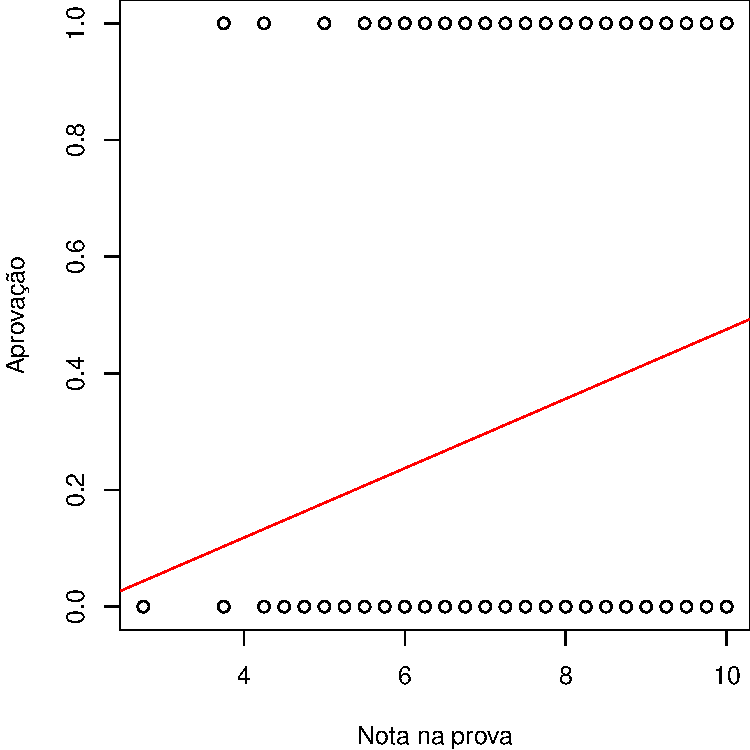
\includegraphics[width=0.6\linewidth]{figure/logplot1-1} 

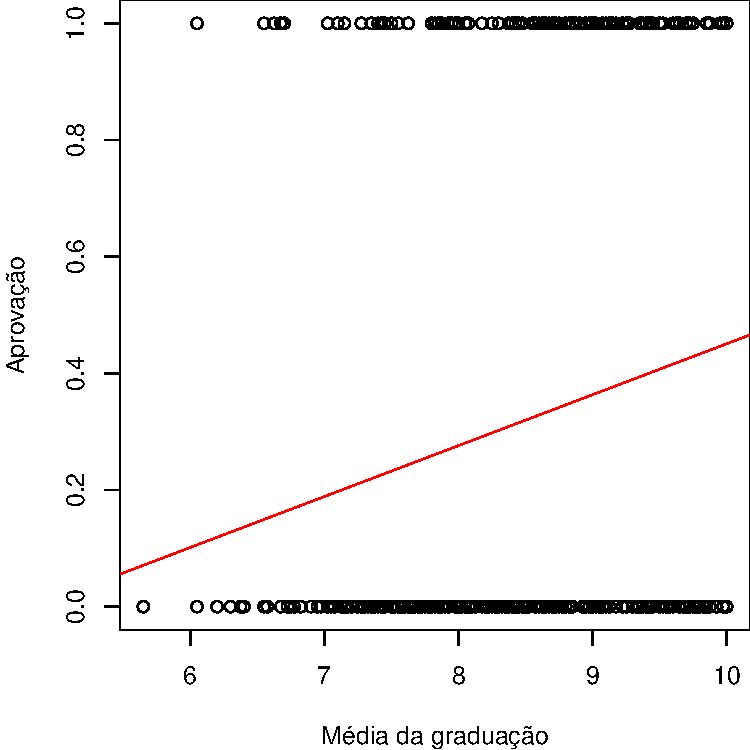
\includegraphics[width=0.6\linewidth]{figure/logplot1-2} 

\end{knitrout}

\end{columns}

\end{frame}
%===============================================================================%

%===============================================================================%
\begin{frame}[fragile]{Regressão Logística}

\begin{columns}

\column{0.7\linewidth}
\setlength{\topsep}{2pt}
\begin{knitrout}\tiny
\definecolor{shadecolor}{rgb}{0.969, 0.969, 0.969}\color{fgcolor}\begin{kframe}
\begin{alltt}
\hlstd{phd} \hlkwb{<-} \hlkwd{read.csv}\hlstd{(}\hlstr{'inpe_aprov_fake.csv'}\hlstd{)}
\hlkwd{head}\hlstd{(phd)}
\hlkwd{par}\hlstd{(}\hlkwc{mar}\hlstd{=}\hlkwd{c}\hlstd{(}\hlnum{7}\hlstd{,}\hlnum{2}\hlstd{,}\hlnum{1}\hlstd{,}\hlnum{0}\hlstd{))}
\hlkwd{boxplot}\hlstd{(prova} \hlopt{~} \hlkwd{factor}\hlstd{(aprovado),} \hlkwc{data}\hlstd{=phd,}\hlkwc{xlab}\hlstd{=}\hlstr{"Prova"}\hlstd{,}\hlkwc{horizontal}\hlstd{=}\hlnum{TRUE}\hlstd{)}
\hlkwd{boxplot}\hlstd{(grad} \hlopt{~}\hlkwd{factor}\hlstd{(aprovado),} \hlkwc{data}\hlstd{=phd,}\hlkwc{xlab}\hlstd{=}\hlstr{"Graduação"}\hlstd{,} \hlkwc{horizontal}\hlstd{=}\hlnum{TRUE}\hlstd{)}
\hlkwd{boxplot}\hlstd{(reco} \hlopt{~} \hlkwd{factor}\hlstd{(aprovado),} \hlkwc{data}\hlstd{=phd,}\hlkwc{horizontal}\hlstd{=}\hlnum{TRUE}\hlstd{,}\hlkwc{xlab}\hlstd{=}\hlstr{"Recomendação"}\hlstd{)}
\end{alltt}
\end{kframe}
\end{knitrout}

\column{0.4\linewidth}
\begin{knitrout}
\definecolor{shadecolor}{rgb}{0.969, 0.969, 0.969}\color{fgcolor}
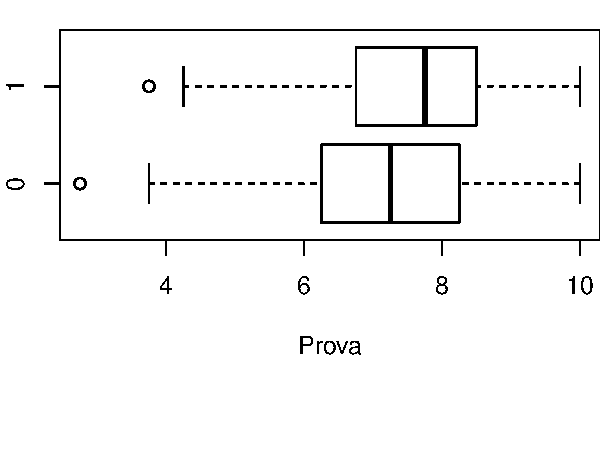
\includegraphics[width=0.6\linewidth]{figure/logplot2-1} 

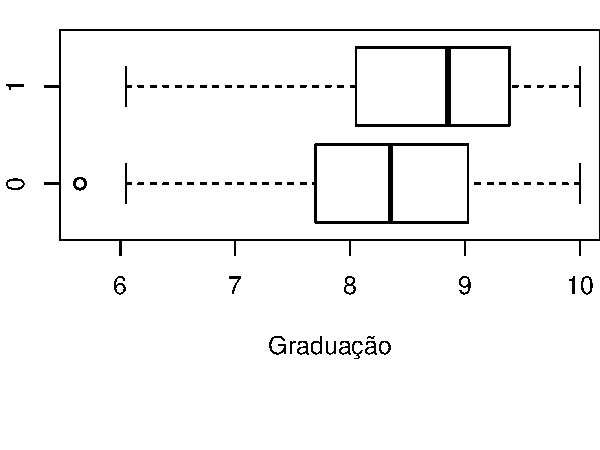
\includegraphics[width=0.6\linewidth]{figure/logplot2-2} 

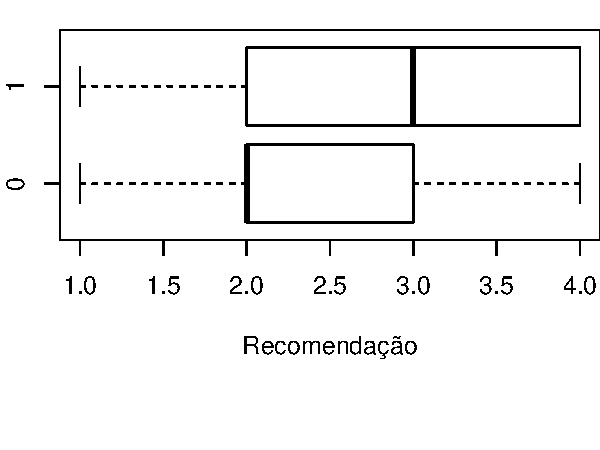
\includegraphics[width=0.6\linewidth]{figure/logplot2-3} 

\end{knitrout}

\end{columns}

\end{frame}
%===============================================================================%


%===============================================================================%
\begin{frame}[fragile]{Regressão Logística}

\begin{columns}

\column{0.7\linewidth}
\setlength{\topsep}{2pt}
\begin{knitrout}\tiny
\definecolor{shadecolor}{rgb}{0.969, 0.969, 0.969}\color{fgcolor}\begin{kframe}
\begin{alltt}
\hlstd{m} \hlkwb{<-} \hlkwd{glm}\hlstd{(aprovado} \hlopt{~} \hlstd{prova, phd,} \hlkwc{family}\hlstd{=}\hlstr{'binomial'}\hlstd{)}
\hlkwd{summary}\hlstd{(m)}
\end{alltt}
\begin{verbatim}
## 
## Call:
## glm(formula = aprovado ~ prova, family = "binomial", data = phd)
## 
## Deviance Residuals: 
##     Min       1Q   Median       3Q      Max  
## -1.1623  -0.9052  -0.7547   1.3486   1.9879  
## 
## Coefficients:
##             Estimate Std. Error z value Pr(>|z|)    
## (Intercept) -2.90134    0.60604  -4.787 1.69e-06 ***
## prova        0.28658    0.07888   3.633  0.00028 ***
## ---
## Signif. codes:  0 '***' 0.001 '**' 0.01 '*' 0.05 '.' 0.1 ' ' 1
## 
## (Dispersion parameter for binomial family taken to be 1)
## 
##     Null deviance: 499.98  on 399  degrees of freedom
## Residual deviance: 486.06  on 398  degrees of freedom
## AIC: 490.06
## 
## Number of Fisher Scoring iterations: 4
\end{verbatim}
\end{kframe}
\end{knitrout}

\column{0.4\linewidth}
\begin{knitrout}
\definecolor{shadecolor}{rgb}{0.969, 0.969, 0.969}\color{fgcolor}
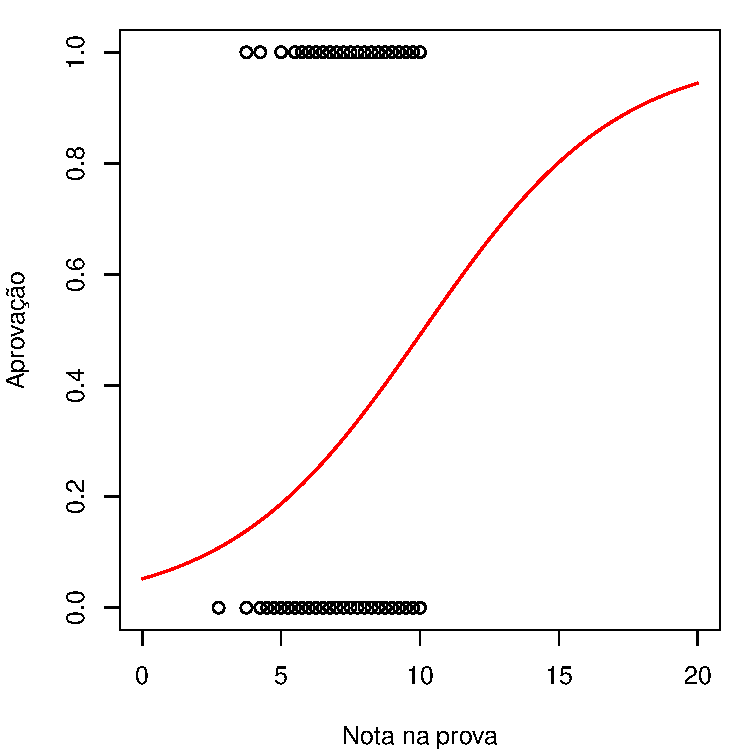
\includegraphics[width=0.8\linewidth]{figure/logplot3-1} 

\end{knitrout}

\end{columns}

\end{frame}
%===============================================================================%


%===============================================================================%
\begin{frame}[fragile]{Regressão Logística}

\begin{columns}

\column{0.7\linewidth}
\setlength{\topsep}{2pt}
\begin{knitrout}\tiny
\definecolor{shadecolor}{rgb}{0.969, 0.969, 0.969}\color{fgcolor}\begin{kframe}
\begin{alltt}
\hlstd{m} \hlkwb{<-} \hlkwd{glm}\hlstd{(aprovado} \hlopt{~} \hlstd{grad, phd,} \hlkwc{family}\hlstd{=}\hlstr{'binomial'}\hlstd{)}
\hlkwd{summary}\hlstd{(m)}
\end{alltt}
\begin{verbatim}
## 
## Call:
## glm(formula = aprovado ~ grad, family = "binomial", data = phd)
## 
## Deviance Residuals: 
##     Min       1Q   Median       3Q      Max  
## -1.1131  -0.8874  -0.7566   1.3305   1.9824  
## 
## Coefficients:
##             Estimate Std. Error z value Pr(>|z|)    
## (Intercept)  -4.3576     1.0353  -4.209 2.57e-05 ***
## grad          0.4204     0.1195   3.517 0.000437 ***
## ---
## Signif. codes:  0 '***' 0.001 '**' 0.01 '*' 0.05 '.' 0.1 ' ' 1
## 
## (Dispersion parameter for binomial family taken to be 1)
## 
##     Null deviance: 499.98  on 399  degrees of freedom
## Residual deviance: 486.97  on 398  degrees of freedom
## AIC: 490.97
## 
## Number of Fisher Scoring iterations: 4
\end{verbatim}
\end{kframe}
\end{knitrout}

\column{0.4\linewidth}
\begin{knitrout}
\definecolor{shadecolor}{rgb}{0.969, 0.969, 0.969}\color{fgcolor}
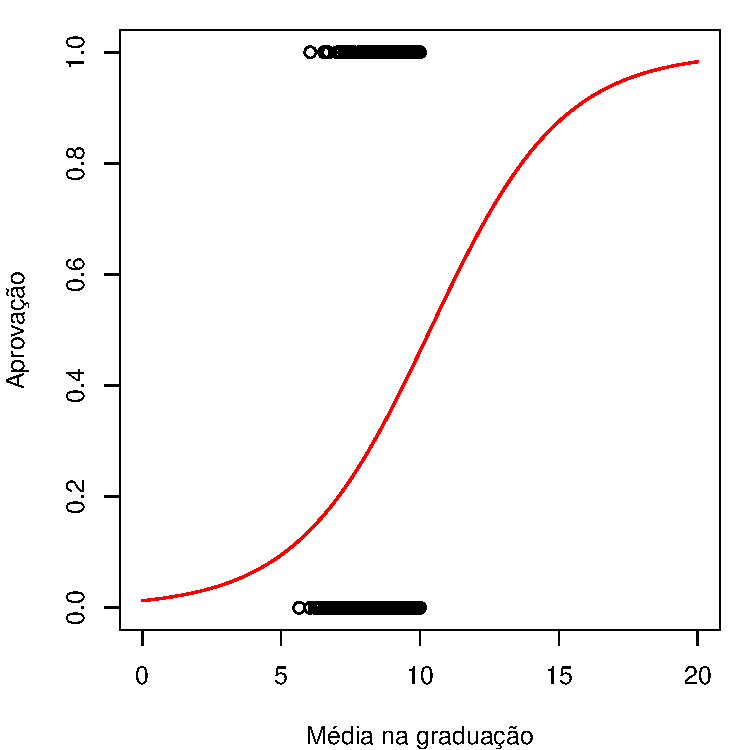
\includegraphics[width=0.8\linewidth]{figure/logplot4-1} 

\end{knitrout}

\end{columns}

\end{frame}
%===============================================================================%


%===============================================================================%
\begin{frame}[fragile]{Regressão Logística}

\begin{columns}

\column{0.7\linewidth}
\setlength{\topsep}{2pt}
\begin{knitrout}\tiny
\definecolor{shadecolor}{rgb}{0.969, 0.969, 0.969}\color{fgcolor}\begin{kframe}
\begin{alltt}
\hlstd{m} \hlkwb{<-} \hlkwd{glm}\hlstd{(aprovado} \hlopt{~} \hlstd{reco, phd,} \hlkwc{family}\hlstd{=}\hlstr{'binomial'}\hlstd{)}
\hlkwd{summary}\hlstd{(m)}
\end{alltt}
\begin{verbatim}
## 
## Call:
## glm(formula = aprovado ~ reco, family = "binomial", data = phd)
## 
## Deviance Residuals: 
##     Min       1Q   Median       3Q      Max  
## -1.1989  -0.9599  -0.7508   1.1561   1.9365  
## 
## Coefficients:
##             Estimate Std. Error z value Pr(>|z|)    
## (Intercept)  -2.2948     0.3524  -6.511 7.46e-11 ***
## reco          0.5863     0.1240   4.728 2.26e-06 ***
## ---
## Signif. codes:  0 '***' 0.001 '**' 0.01 '*' 0.05 '.' 0.1 ' ' 1
## 
## (Dispersion parameter for binomial family taken to be 1)
## 
##     Null deviance: 499.98  on 399  degrees of freedom
## Residual deviance: 475.71  on 398  degrees of freedom
## AIC: 479.71
## 
## Number of Fisher Scoring iterations: 4
\end{verbatim}
\end{kframe}
\end{knitrout}

\column{0.4\linewidth}
\begin{knitrout}
\definecolor{shadecolor}{rgb}{0.969, 0.969, 0.969}\color{fgcolor}
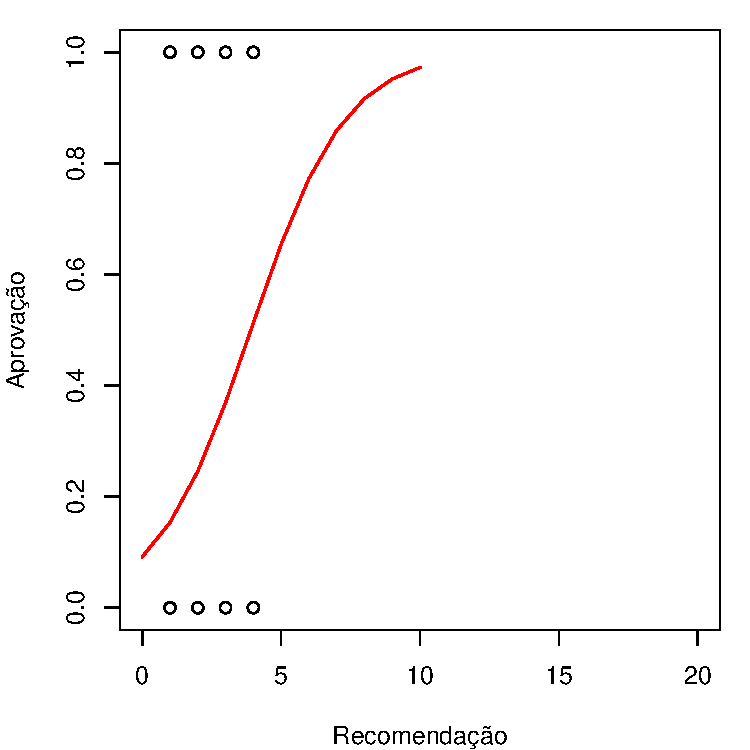
\includegraphics[width=0.8\linewidth]{figure/logplot5-1} 

\end{knitrout}

\end{columns}

\end{frame}
%===============================================================================%

%===============================================================================%
\begin{frame}[fragile]{Regressão Logística}

\begin{columns}

\column{0.7\linewidth}
\setlength{\topsep}{2pt}

\begin{knitrout}\tiny
\definecolor{shadecolor}{rgb}{0.969, 0.969, 0.969}\color{fgcolor}\begin{kframe}
\begin{alltt}
\hlstd{m} \hlkwb{<-} \hlkwd{glm}\hlstd{(aprovado} \hlopt{~} \hlstd{grad} \hlopt{+} \hlstd{prova} \hlopt{+} \hlstd{reco, phd,} \hlkwc{family}\hlstd{=}\hlstr{'binomial'}\hlstd{)}
\hlkwd{summary}\hlstd{(m)}
\end{alltt}
\begin{verbatim}
## 
## Call:
## glm(formula = aprovado ~ grad + prova + reco, family = "binomial", 
##     data = phd)
## 
## Deviance Residuals: 
##     Min       1Q   Median       3Q      Max  
## -1.5802  -0.8848  -0.6382   1.1575   2.1732  
## 
## Coefficients:
##             Estimate Std. Error z value Pr(>|z|)    
## (Intercept) -6.24971    1.15573  -5.408 6.39e-08 ***
## grad         0.31081    0.13099   2.373   0.0177 *  
## prova        0.18352    0.08735   2.101   0.0356 *  
## reco         0.56003    0.12714   4.405 1.06e-05 ***
## ---
## Signif. codes:  0 '***' 0.001 '**' 0.01 '*' 0.05 '.' 0.1 ' ' 1
## 
## (Dispersion parameter for binomial family taken to be 1)
## 
##     Null deviance: 499.98  on 399  degrees of freedom
## Residual deviance: 459.44  on 396  degrees of freedom
## AIC: 467.44
## 
## Number of Fisher Scoring iterations: 4
\end{verbatim}
\end{kframe}
\end{knitrout}

\column{0.4\linewidth}
\begin{knitrout}\tiny
\definecolor{shadecolor}{rgb}{0.969, 0.969, 0.969}\color{fgcolor}\begin{kframe}
\begin{alltt}
\hlcom{# exponencial dos coeficientes = odds}
\hlkwd{exp}\hlstd{(m}\hlopt{$}\hlstd{coefficients[}\hlnum{2}\hlopt{:}\hlnum{4}\hlstd{])}
\end{alltt}
\begin{verbatim}
##     grad    prova     reco 
## 1.364524 1.201435 1.750727
\end{verbatim}
\end{kframe}
\end{knitrout}

\end{columns}

\end{frame}
%===============================================================================%


%===============================================================================%
\begin{frame}{Modelos Lineares Generalizados}

A regressão logística é um caso específico dos chamados \textbf{Modelos Lineares \emph{Generalizados}}
\vfill
\begin{itemize}
\item Estendem os modelos lineares gerais para dados não-normais
\vfill
\item Utilizam a chamada \emph{função link} para relacionar os dados originais com uma distribuição normal
\end{itemize}

\begin{center}
\begin{tabular}{l{5cm} l}
\hline
Função Link & Distribuições \\
\hline
Identidade & Normal \\
Inversa & Exponencial, Gamma \\
Log & Poisson \\
Logito & Bernoulli, Binomial, Multinomial \\
\hline
\end{tabular}
\end{center}

\end{frame}
%===============================================================================%

%===============================================================================%
\begin{frame}{Extendendo os modelos lineares: Generalized Linear Models}

Dúvida: usar uma função link não é a mesma coisa que transformar a variável? \pause
\vfill
\begin{itemize}
\item Não exatamente. A função link transforma $E(Y)$, e não $Y$ \pause
\vfill
\item Por exemplo: Função Log
\vfill
\begin{itemize}
\item Se você transforma a variável, está estimando $E(log(Y))$ \pause
\vfill
\item Um GLM com função link estima $log(E(Y))$ \pause
\vfill
\end{itemize}
\item Os parâmetros serão diferentes, e o GLM produz estimativas mais precisas
\end{itemize}

\end{frame}
%===============================================================================%

\section{Mínimos Quadrados Generalizados}

%===============================================================================%
\begin{frame}{Mínimos Quadrados Generalizados}

Método generalizado de mínimos quadrados para o ajuste de modelos
\vfill
\begin{itemize}
\item Generalized Least Squares (GLS) $\ne$ Generalized Linear Model (GLM)
\vfill
\item Permite estimar parâmetros quando os resíduos são heteroscedásticos
\vfill
\item Permite estimar parâmetros quando os resíduos são correlacionados
\vfill
\end{itemize}

\end{frame}
%===============================================================================%


%===============================================================================%
\begin{frame}{Mínimos Quadrados Generalizados}

Na regressão por mínimos quadrados ordinários (OLS), assumimos que $e \sim N(0,s^2)$
\vfill
Como poderíamos modificar a descrição de $e$, para dados onde a variância cresce com os valores de $X$? \pause
\vfill
$e \sim N(0,s^2 \times X)$: modelo fixo de estrutura de variância \pause


\end{frame}
%===============================================================================%


%===============================================================================%
\begin{frame}{Mínimos Quadrados Generalizados}

Poderiam haver outros tipos de relação entre $Var(e)$ e $X$? \pause

\small
\vfill
$e \sim N(0,s^2_j)$: modelo VarIdent de estrutura de variânica ($X$ categórico) \pause
\vfill
$e \sim N(0,s^2 \times \lvert X_j \rvert ^{2\delta})$: modelo VarPower (não funciona se $X$ tem zeros) \pause
\vfill
$e \sim N(0,s^2 \times e^{2\delta \times X})$: modelo VarExp (funciona se $X$ tem zeros) \pause
\vfill
$e \sim N(0,s^2 \times (\delta_1 \times \lvert X \rvert ^{2\delta_2})^2)$: modelo VarConstPower \pause
\vfill
$e \sim N(0,s^2_j \times e^{2\delta_2 \times X})$: modelo VarComb \pause
\vfill
\scriptsize
Para saber mais: Zuur et al. (2009). Mixed effects models and extensions in Ecology with R. Springer.

\end{frame}
%===============================================================================%

%===============================================================================%
\begin{frame}[fragile]{GLS}

\begin{columns}[c]

\column{0.7\linewidth}
\setlength{\topsep}{2pt}
\begin{knitrout}\tiny
\definecolor{shadecolor}{rgb}{0.969, 0.969, 0.969}\color{fgcolor}\begin{kframe}
\begin{alltt}
\hlcom{# Exemplo de Zuur et al. (2009)m - Lulas <- }
\hlkwd{library}\hlstd{(nlme)}
\hlstd{Squid}\hlkwb{<-}\hlkwd{read.table}\hlstd{(}\hlkwc{file}\hlstd{=}\hlstr{"Squid.txt"}\hlstd{,}\hlkwc{header}\hlstd{=}\hlnum{TRUE}\hlstd{)}
\hlstd{Squid}\hlopt{$}\hlstd{fMONTH}\hlkwb{=}\hlkwd{factor}\hlstd{(Squid}\hlopt{$}\hlstd{MONTH)}
\hlstd{M1} \hlkwb{<-} \hlkwd{lm}\hlstd{(Testisweight} \hlopt{~} \hlstd{DML} \hlopt{*} \hlstd{fMONTH,}\hlkwc{data}\hlstd{=Squid)}
\hlkwd{anova}\hlstd{(M1)}
\end{alltt}
\begin{verbatim}
## Analysis of Variance Table
## 
## Response: Testisweight
##             Df  Sum Sq Mean Sq  F value    Pr(>F)    
## DML          1 11247.2 11247.2 1732.082 < 2.2e-16 ***
## fMONTH      11  2099.1   190.8   29.388 < 2.2e-16 ***
## DML:fMONTH  11  1678.0   152.5   23.492 < 2.2e-16 ***
## Residuals  744  4831.1     6.5                       
## ---
## Signif. codes:  0 '***' 0.001 '**' 0.01 '*' 0.05 '.' 0.1 ' ' 1
\end{verbatim}
\end{kframe}
\end{knitrout}

\column{0.4\linewidth}
\begin{knitrout}
\definecolor{shadecolor}{rgb}{0.969, 0.969, 0.969}\color{fgcolor}
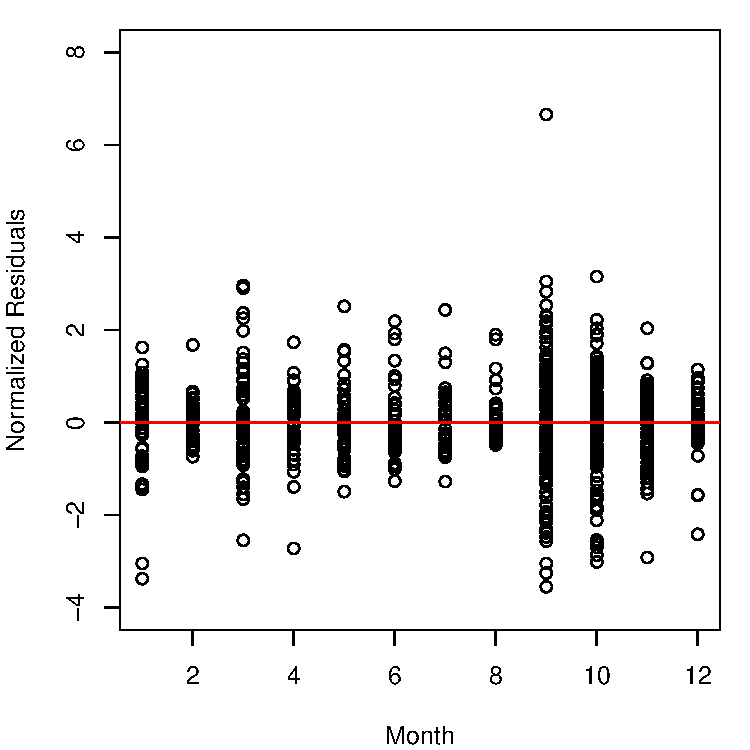
\includegraphics[width=0.7\linewidth]{figure/glsp1-1} 

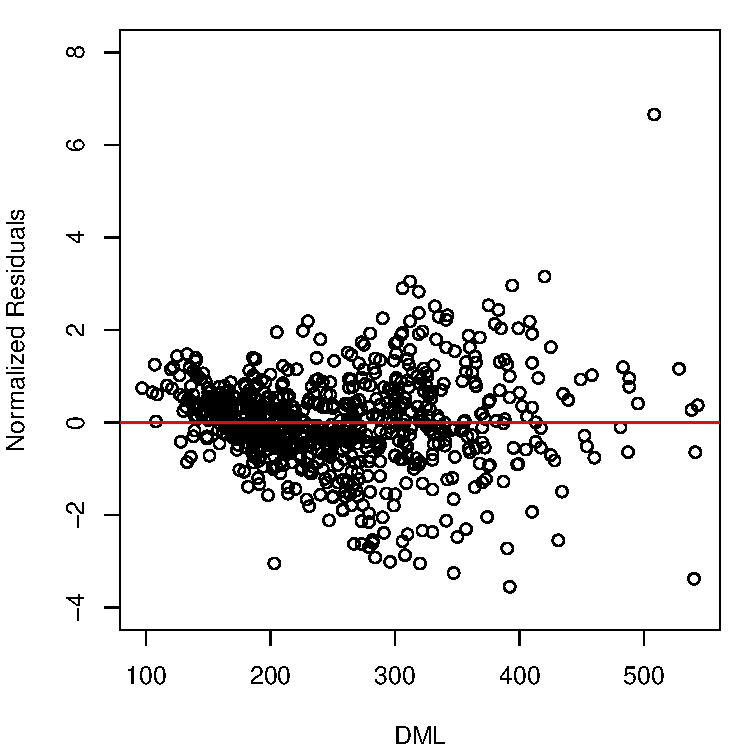
\includegraphics[width=0.7\linewidth]{figure/glsp1-2} 

\end{knitrout}

\end{columns}

\end{frame}
%===============================================================================%


%===============================================================================%
\begin{frame}[fragile]{GLS}

\begin{columns}[c]

\column{0.7\linewidth}
\setlength{\topsep}{2pt}
\begin{knitrout}\tiny
\definecolor{shadecolor}{rgb}{0.969, 0.969, 0.969}\color{fgcolor}\begin{kframe}
\begin{alltt}
\hlcom{# Usando VarIdent para corrigir o efeito de DML}
\hlstd{M.lm}\hlkwb{<-}\hlkwd{gls}\hlstd{(Testisweight}\hlopt{~}\hlstd{DML}\hlopt{*}\hlstd{fMONTH,}\hlkwc{data}\hlstd{=Squid)}
\hlstd{M.gls1}\hlkwb{<-}\hlkwd{gls}\hlstd{(Testisweight}\hlopt{~}\hlstd{DML}\hlopt{*}\hlstd{fMONTH,}\hlkwc{weights}\hlstd{=}\hlkwd{varFixed}\hlstd{(}\hlopt{~}\hlstd{DML),}\hlkwc{data}\hlstd{=Squid)}
\hlkwd{AIC}\hlstd{(M.lm,M.gls1)}
\end{alltt}
\begin{verbatim}
##        df      AIC
## M.lm   25 3752.084
## M.gls1 25 3620.898
\end{verbatim}
\end{kframe}
\end{knitrout}

\column{0.4\linewidth}
\begin{knitrout}
\definecolor{shadecolor}{rgb}{0.969, 0.969, 0.969}\color{fgcolor}
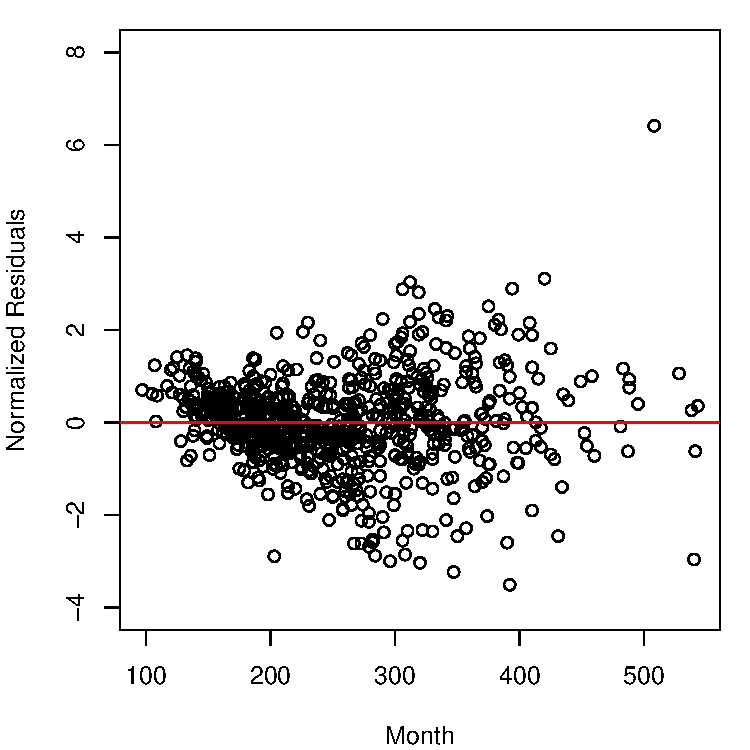
\includegraphics[width=0.7\linewidth]{figure/glsp2-1} 

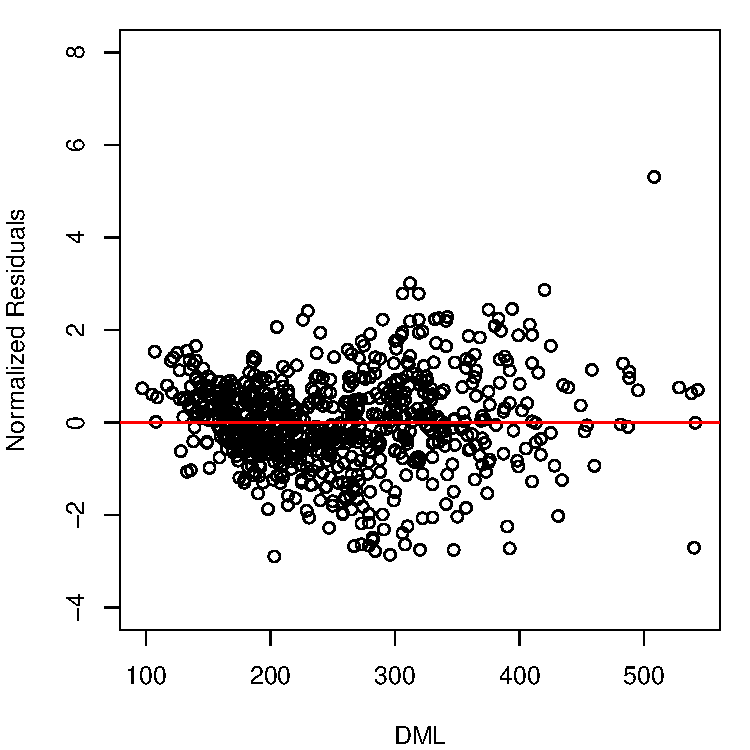
\includegraphics[width=0.7\linewidth]{figure/glsp2-2} 

\end{knitrout}

\end{columns}

\end{frame}
%===============================================================================%

%===============================================================================%
\begin{frame}[fragile]{GLS}

\begin{columns}[c]

\column{0.7\linewidth}
\setlength{\topsep}{2pt}
\begin{knitrout}\tiny
\definecolor{shadecolor}{rgb}{0.969, 0.969, 0.969}\color{fgcolor}\begin{kframe}
\begin{alltt}
\hlcom{# Usando VarIdent para corrigir o efeito de DML}
\hlstd{M.gls2} \hlkwb{<-} \hlkwd{gls}\hlstd{(Testisweight} \hlopt{~} \hlstd{DML}\hlopt{*}\hlstd{fMONTH,} \hlkwc{weights}\hlstd{=}\hlkwd{varIdent}\hlstd{(}\hlkwc{form}\hlstd{=} \hlopt{~} \hlnum{1}\hlopt{|}\hlstd{fMONTH),} \hlkwc{data} \hlstd{=Squid)}
\hlkwd{AIC}\hlstd{(M.lm,M.gls1,M.gls2)}
\end{alltt}
\begin{verbatim}
##        df      AIC
## M.lm   25 3752.084
## M.gls1 25 3620.898
## M.gls2 36 3614.436
\end{verbatim}
\end{kframe}
\end{knitrout}

\column{0.4\linewidth}
\begin{knitrout}
\definecolor{shadecolor}{rgb}{0.969, 0.969, 0.969}\color{fgcolor}
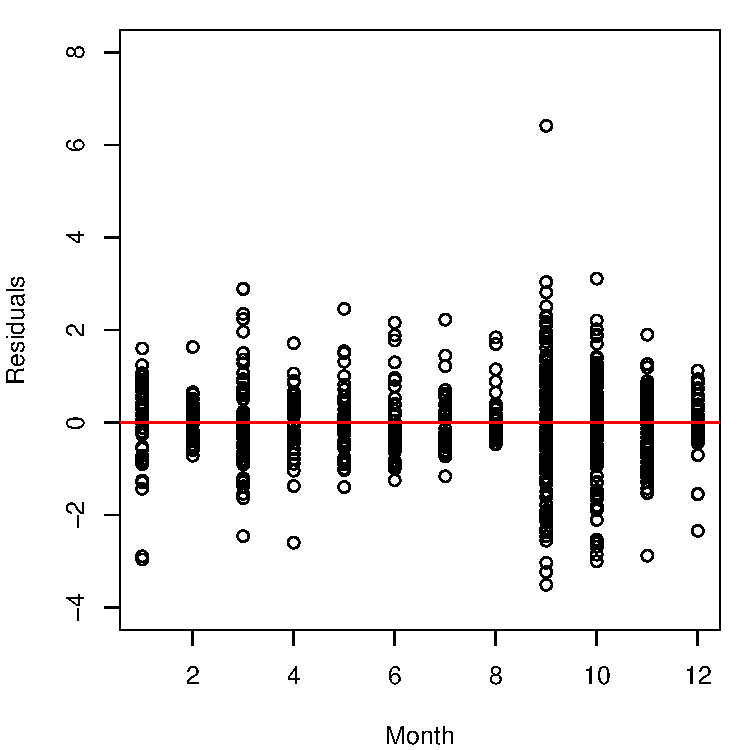
\includegraphics[width=0.7\linewidth]{figure/glsp3-1} 

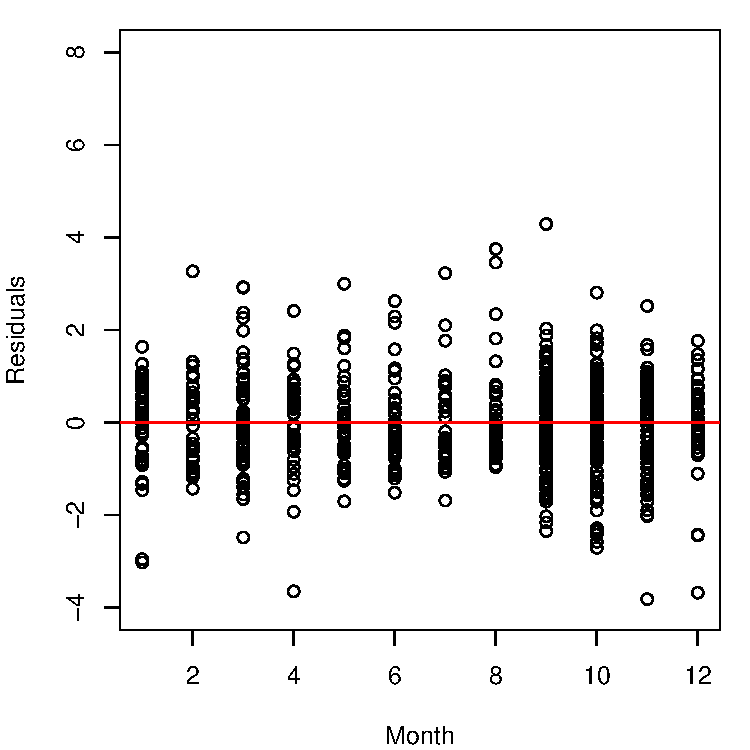
\includegraphics[width=0.7\linewidth]{figure/glsp3-2} 

\end{knitrout}

\end{columns}

\end{frame}
%===============================================================================%


%===============================================================================%
\begin{frame}[fragile]{GLS}

\begin{columns}[c]

\column{0.7\linewidth}
\setlength{\topsep}{2pt}
\begin{knitrout}\tiny
\definecolor{shadecolor}{rgb}{0.969, 0.969, 0.969}\color{fgcolor}\begin{kframe}
\begin{alltt}
\hlcom{# Usando VarPower para corrigir o efeito de DML e MONTH}
\hlstd{M.gls3}\hlkwb{<-}\hlkwd{gls}\hlstd{(Testisweight} \hlopt{~} \hlstd{DML} \hlopt{*} \hlstd{fMONTH,} \hlkwc{data} \hlstd{= Squid,}\hlkwc{weights} \hlstd{=} \hlkwd{varPower}\hlstd{(}\hlkwc{form}\hlstd{=}\hlopt{~} \hlstd{DML} \hlopt{|} \hlstd{fMONTH))}
\hlkwd{AIC}\hlstd{(M.lm,M.gls1,M.gls2,M.gls3)}
\end{alltt}
\begin{verbatim}
##        df      AIC
## M.lm   25 3752.084
## M.gls1 25 3620.898
## M.gls2 36 3614.436
## M.gls3 37 3407.511
\end{verbatim}
\end{kframe}
\end{knitrout}

\column{0.4\linewidth}
\begin{knitrout}
\definecolor{shadecolor}{rgb}{0.969, 0.969, 0.969}\color{fgcolor}
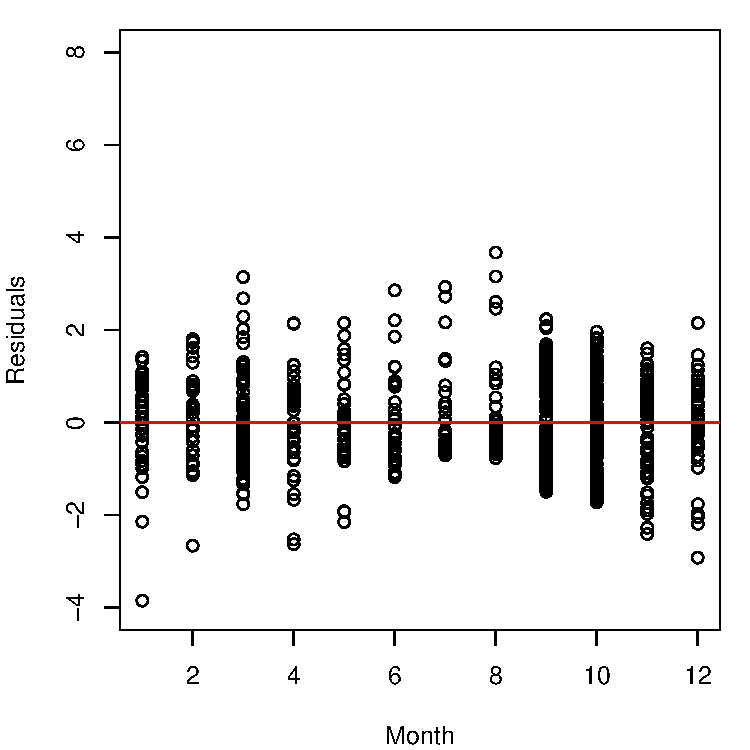
\includegraphics[width=0.7\linewidth]{figure/glsp4-1} 

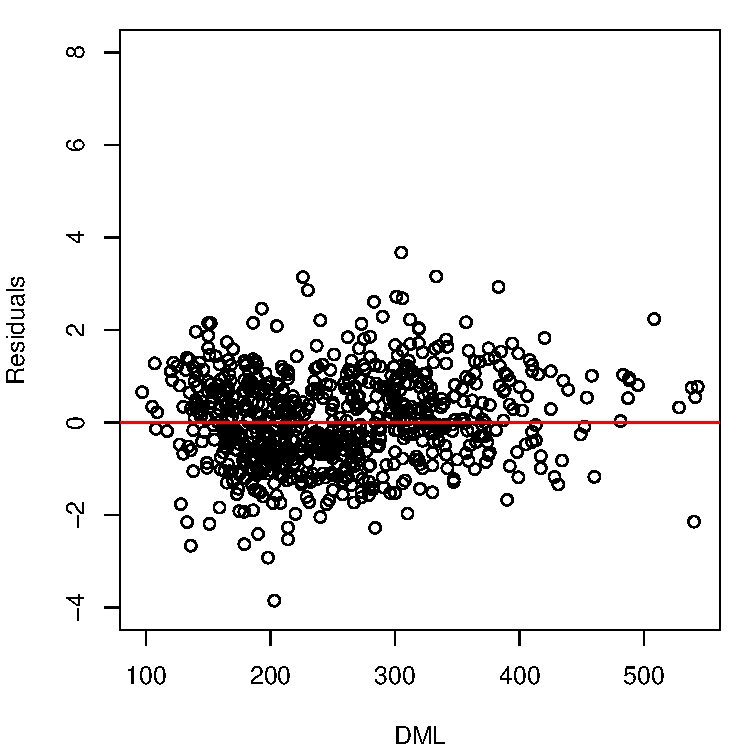
\includegraphics[width=0.7\linewidth]{figure/glsp4-2} 

\end{knitrout}

\end{columns}

\end{frame}
%===============================================================================%


%===============================================================================%
\begin{frame}[fragile]{GLS}

 Resíduos no modelo estimado por OLS

\begin{knitrout}
\definecolor{shadecolor}{rgb}{0.969, 0.969, 0.969}\color{fgcolor}
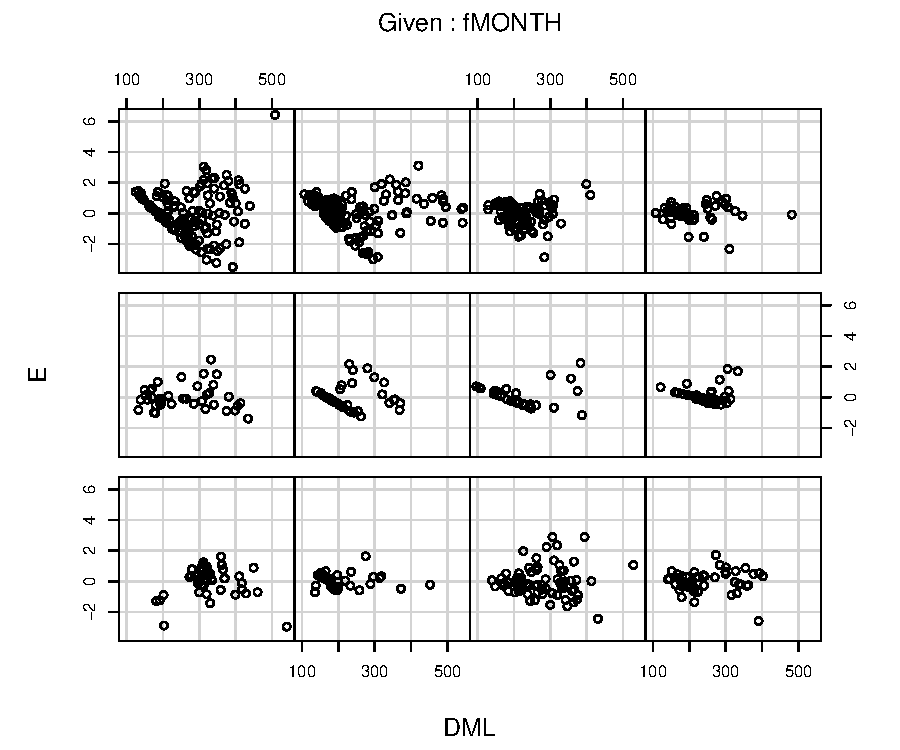
\includegraphics[width=0.7\linewidth]{figure/glsp5-1} 

\end{knitrout}


\end{frame}
%===============================================================================%

%===============================================================================%
\begin{frame}[fragile]{GLS}

 GLS com varPower(form=~ DML | fMONTH)

\begin{knitrout}
\definecolor{shadecolor}{rgb}{0.969, 0.969, 0.969}\color{fgcolor}
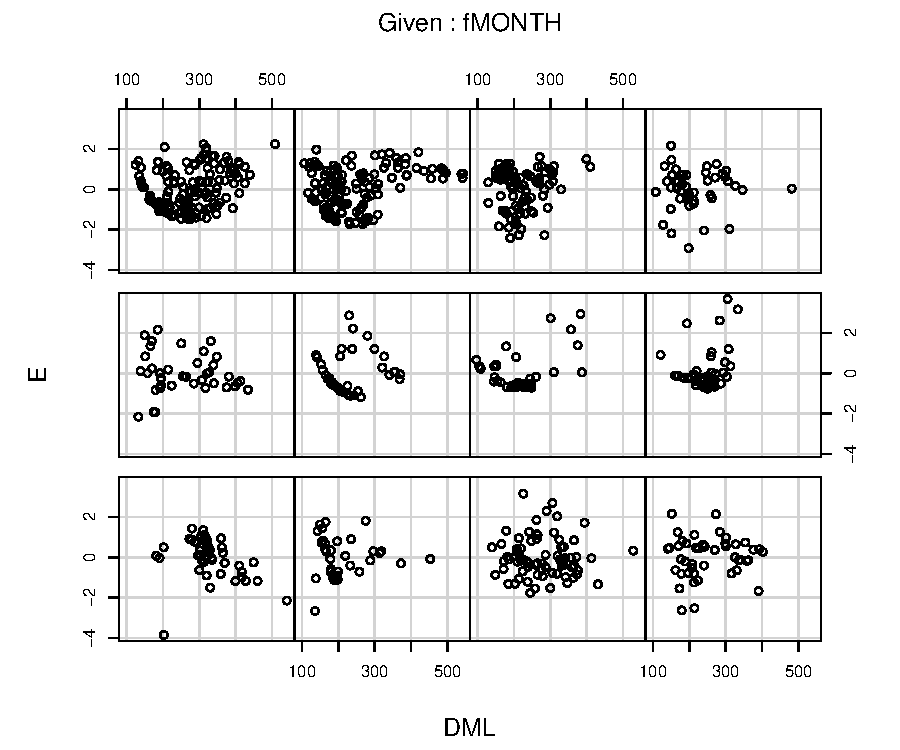
\includegraphics[width=0.7\linewidth]{figure/glsp6-1} 

\end{knitrout}


\end{frame}
%===============================================================================%


%===============================================================================%
\begin{frame}{Mínimos Quadrados Generalizados}

Como poderíamos modificar a descrição de $e$, para dados onde os valores são correlacionados? \pause
\vfill
$e \sim N(0,\rho \times s^2 )$: modelo de correlação simétrico 
\vfill 
$\rho$ é a correlação entre $X_i$ e $X_{j\ne i}$ \pause
\vfill
$e \sim N(0,\rho \times s^2 )$: modelo de correlação autoregressivo (AR) de ordem 1
\vfill 
cor($X_i$,$X_{i-1}$) = $\rho$;  cor($X_i$,$X_{i-2}$) = $\rho ^2$; cor($X_i$,$X_{i-n}$) = $\rho ^n$ \pause
\vfill
Existem modelos (bem) mais complexos.

\end{frame}
%===============================================================================%

%===============================================================================%
\begin{frame}[fragile]{GLS}

\begin{columns}[c]

\column{0.7\linewidth}
\setlength{\topsep}{2pt}
\begin{knitrout}\tiny
\definecolor{shadecolor}{rgb}{0.969, 0.969, 0.969}\color{fgcolor}\begin{kframe}
\begin{alltt}
\hlcom{# Exemplo de Zuur et al. (2009)m - Pássaros  }
\hlstd{Hawaii}\hlkwb{<-}\hlkwd{read.table}\hlstd{(}\hlkwc{file}\hlstd{=}\hlstr{"Hawaii.txt"}\hlstd{,}\hlkwc{header}\hlstd{=}\hlnum{TRUE}\hlstd{)}
\hlstd{Hawaii}\hlopt{$}\hlstd{Birds}\hlkwb{<-}\hlkwd{sqrt}\hlstd{(Hawaii}\hlopt{$}\hlstd{Moorhen.Kauai)}
\hlstd{M0} \hlkwb{<-} \hlkwd{gls}\hlstd{(Birds} \hlopt{~} \hlstd{Rainfall} \hlopt{+} \hlstd{Year,} \hlkwc{na.action} \hlstd{= na.omit,} \hlkwc{data} \hlstd{= Hawaii)}
\end{alltt}
\end{kframe}
\end{knitrout}

\column{0.4\linewidth}
\begin{knitrout}
\definecolor{shadecolor}{rgb}{0.969, 0.969, 0.969}\color{fgcolor}
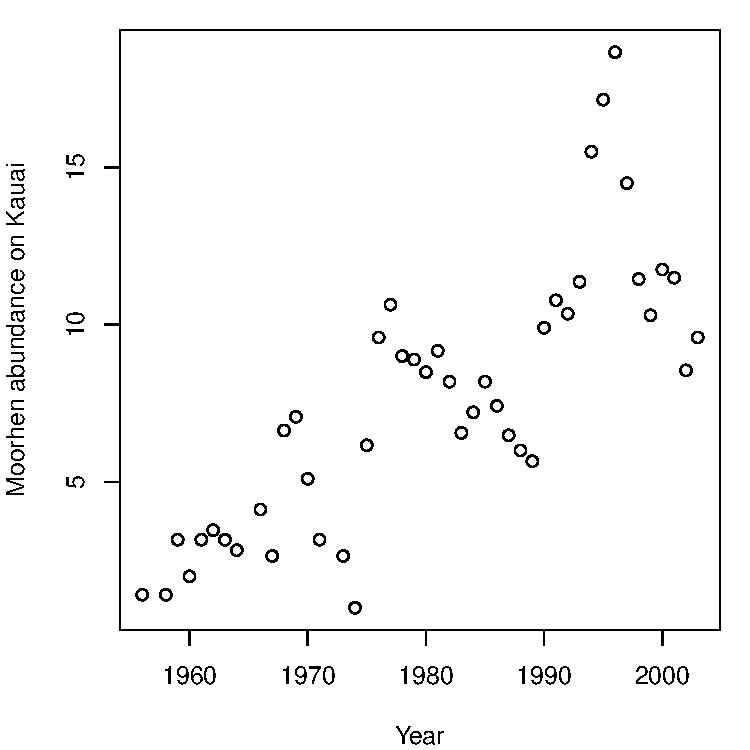
\includegraphics[width=0.7\linewidth]{figure/glspt1-1} 

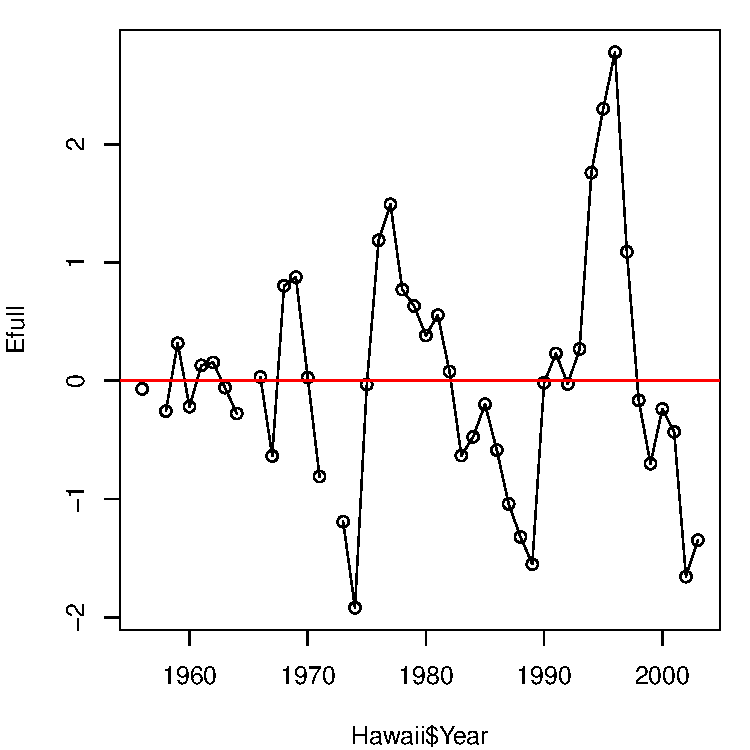
\includegraphics[width=0.7\linewidth]{figure/glspt1-2} 

\end{knitrout}

\end{columns}

\end{frame}
%===============================================================================%



%===============================================================================%
\begin{frame}[fragile]{GLS}

\begin{columns}[c]

\column{0.7\linewidth}
\setlength{\topsep}{2pt}
\begin{knitrout}\tiny
\definecolor{shadecolor}{rgb}{0.969, 0.969, 0.969}\color{fgcolor}\begin{kframe}
\begin{alltt}
\hlcom{# Exemplo de Zuur et al. (2009)m - Pássaros  }
\hlstd{Hawaii}\hlkwb{<-}\hlkwd{read.table}\hlstd{(}\hlkwc{file}\hlstd{=}\hlstr{"Hawaii.txt"}\hlstd{,}\hlkwc{header}\hlstd{=}\hlnum{TRUE}\hlstd{)}
\hlstd{Hawaii}\hlopt{$}\hlstd{Birds}\hlkwb{<-}\hlkwd{sqrt}\hlstd{(Hawaii}\hlopt{$}\hlstd{Moorhen.Kauai)}
\hlstd{M0} \hlkwb{<-} \hlkwd{gls}\hlstd{(Birds} \hlopt{~} \hlstd{Rainfall} \hlopt{+} \hlstd{Year,} \hlkwc{na.action} \hlstd{= na.omit,} \hlkwc{data} \hlstd{= Hawaii)}
\end{alltt}
\end{kframe}
\end{knitrout}

\column{0.4\linewidth}
\begin{knitrout}
\definecolor{shadecolor}{rgb}{0.969, 0.969, 0.969}\color{fgcolor}
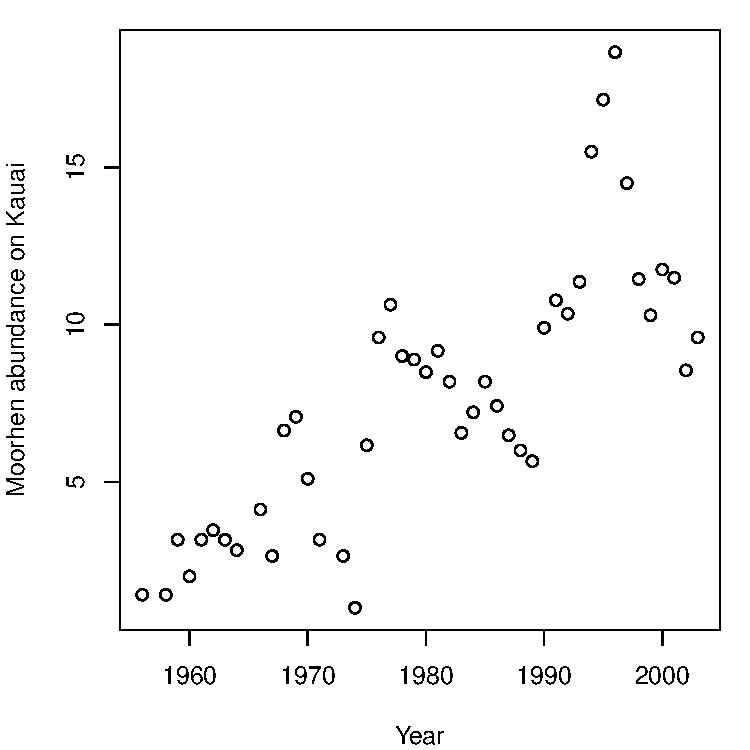
\includegraphics[width=0.7\linewidth]{figure/glspt2-1} 

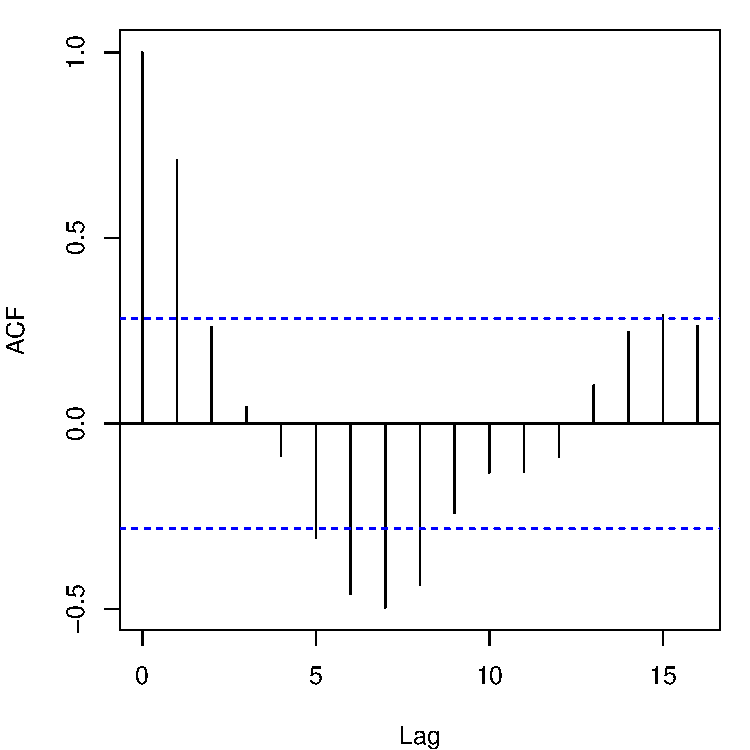
\includegraphics[width=0.7\linewidth]{figure/glspt2-2} 

\end{knitrout}

\end{columns}

\end{frame}
%===============================================================================%


%===============================================================================%
\begin{frame}[fragile]{GLS}

\begin{columns}[c]

\column{0.7\linewidth}
\setlength{\topsep}{2pt}
\begin{knitrout}\tiny
\definecolor{shadecolor}{rgb}{0.969, 0.969, 0.969}\color{fgcolor}\begin{kframe}
\begin{alltt}
\hlcom{# Exemplo de Zuur et al. (2009) - Pássaros  }
\hlstd{M1}\hlkwb{<-}\hlkwd{gls}\hlstd{(Birds} \hlopt{~} \hlstd{Rainfall} \hlopt{+} \hlstd{Year,} \hlkwc{na.action} \hlstd{= na.omit,}
        \hlkwc{correlation} \hlstd{=} \hlkwd{corCompSymm}\hlstd{(}\hlkwc{form} \hlstd{=}\hlopt{~} \hlstd{Year),}
        \hlkwc{data}\hlstd{=Hawaii)}

\hlstd{M2}\hlkwb{<-}\hlkwd{gls}\hlstd{(Birds} \hlopt{~} \hlstd{Rainfall} \hlopt{+} \hlstd{Year,} \hlkwc{na.action} \hlstd{= na.omit,}
      \hlkwc{correlation} \hlstd{=} \hlkwd{corAR1}\hlstd{(}\hlkwc{form} \hlstd{=}\hlopt{~} \hlstd{Year),} \hlkwc{data} \hlstd{= Hawaii)}

\hlkwd{AIC}\hlstd{(M0,M1,M2)}
\end{alltt}
\begin{verbatim}
##    df      AIC
## M0  4 228.4798
## M1  5 230.4798
## M2  5 199.1394
\end{verbatim}
\end{kframe}
\end{knitrout}

\column{0.4\linewidth}
\begin{knitrout}
\definecolor{shadecolor}{rgb}{0.969, 0.969, 0.969}\color{fgcolor}
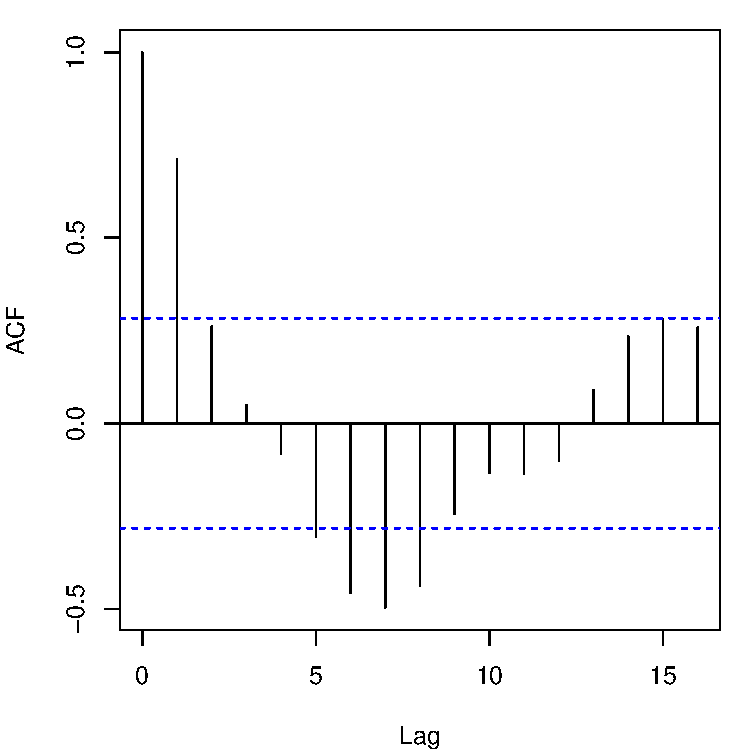
\includegraphics[width=0.7\linewidth]{figure/glspt3-1} 

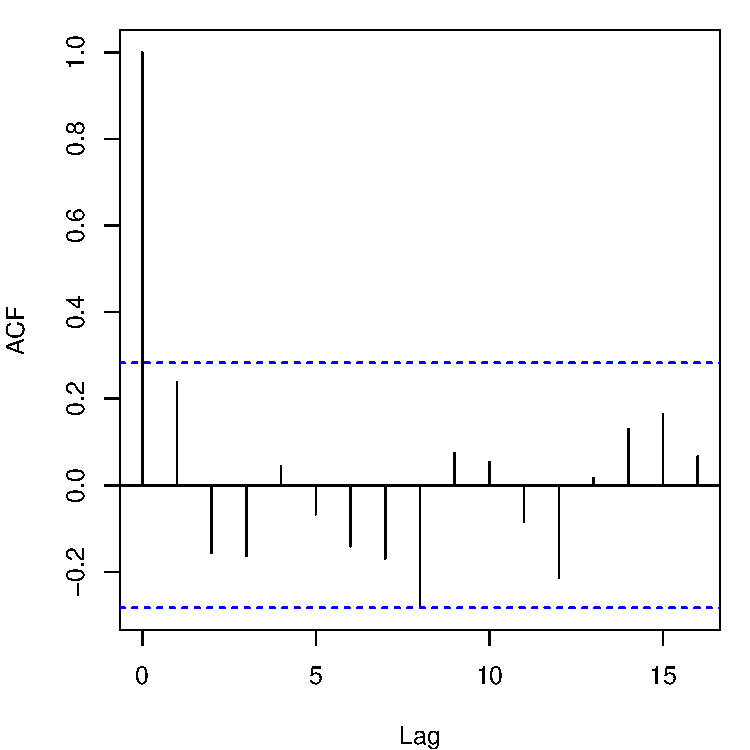
\includegraphics[width=0.7\linewidth]{figure/glspt3-2} 

\end{knitrout}

\end{columns}

\end{frame}
%===============================================================================%


%===============================================================================%
\begin{frame}{Vou ficar devendo \ldots}

Regressão Robusta
\vfill
Regressão por Quantil
\vfill
Regressão Não-Linear
\vfill
Modelos Aditivos Generalizados (Generalized Additive Models, GAM)
\vfill
Splines
\vfill 
Mixed Models


\end{frame}
%===============================================================================%



%===============================================================================%
\begin{frame}{Leituras Recomendadas:}

\begin{scriptsize}

Bolker BM, Brooks ME, Clark CJ, Geange SW, Poulsen JR, Stevens MHH, White J-SS (2009) Generalized linear mixed models: a practical guide for ecology and evolution. Trends in ecology & evolution, 24, 127–35.
\vfill
Yee TW, Mitchell ND (1991) Generalized additive models in plant ecology. Journal of Vegetation Science, 2, 587–602.
\vfill
Zuur A, Ieno E, Walker N, Saveliev A, Smith G (2009) Mixed Effects Models and Extensions in Ecology with R. Springer.
\vfill
Pinheiro J, Bates D (2000) Mixed-Effects Models in S and S-PLUS. Springer.

\end{scriptsize}

\end{frame}
%===============================================================================%

\end{document}
